\chapter{Swiss Terrain 3D}
\label{chap_swiss_terrain_3d}
Kapitel \ref{chap_datengrundlage} behandelte die Datengrundlage für die Terrainvisualisierung. In Kapitel \ref{chap_technologien} wurden Programme und Frameworks zur Erstellung von 3D-Visualisierungen thematisiert. Die technisch notwendigen Grundlagen zur Grafikprogrammierung wurden im Rahmen von Kapitel \ref{chap_render_pipelines} erläutert. Kapitel \ref{chap_algorithmen} befasste sich mit gängigen Datenstrukturen und Algorithmen. Aufbauend auf diesem Vorwissen geht es in diesem Kapitel nun um die eigentliche Implementierung der Terrainvisualisierung.

\section{Technologie und Anforderungen}
\label{technologie_anforderungen}
Bevor eine Visualisierung implementiert werden kann, müssen sowohl die Anforderungen als auch die dafür verwendete Technologie festgelegt werden. Eine echtzeitfähige 3D-Visualisierung ist vereinfacht ausgedrückt eine fortlaufende Abfolge von Bildern, die von der Grafikkarte erzeugt werden. Die Bildgenerierung erfolgt dabei unter Berücksichtigung von Parametern wie  Kameraperspektive, Datenbasis und Interaktion. Damit eine Visualisierung als echtzeitfähig gilt, muss sie mit mindestens 30 Bildern pro Sekunde (FPS) gezeichnet werden. Moderne Monitore unterstützen jedoch deutlich höhere Bildfrequenzen, sodass Darstellungsraten von 60 bis 140 FPS heute keine Seltenheit mehr sind. Neben der Bildrate spielt auch die Auflösung eine entscheidende Rolle. Je höher die Auflösung, desto detailgetreuer lässt sich die Visualisierung darstellen. Sowohl eine hohe Auflösung als auch eine hohe Bildrate erfordern eine entsprechend leistungsfähige Grafikkarte, was den Kreis der potenziellen Zielgruppe einschränken kann. Um einen ausgewogenen Kompromiss zwischen visueller Qualität und breiter Nutzbarkeit zu erreichen, legt diese Masterarbeit daher folgende Mindestanforderung an die Visualisierung fest:\textit{Die Visualisierung soll mit mindestens 60 Bildern pro Sekunde bei einer Auflösung von 2k laufen}.

Nebst den technischen Anforderungen stellt sich auch die Frage, welche Plattformen unterstützt werden sollen. Aktuell sind auf den meisten Betriebssystemen sowie mobilen Endgeräten bereits Browser vorinstalliert. Browserbasierte Anwendungen haben zudem den Vorteil, dass keinerlei Installationsaufwand seitens der Nutzer anfällt. Um eine möglichst breite Zielgruppe ohne Installationsaufwand abzudecken, hat sich der Autor daher für eine webbasierte Implementierung entschieden. 

Wie in Kapitel \ref{chap_technologien} thematisiert, unterstützen moderne Engines wie Unity, Unreal und Godot das Erstellen von browserbasierten Anwendungen. Die primäre Hauptzielgruppe dieser Engines sind jedoch nach wie vor native Anwendungen und Betriebssysteme. Zudem fallen bei kommerziellen Engines wie Unity und Unreal entsprechende Lizenzgebühren an. Obwohl Engines zahlreiche Programme und Editoren bereitstellen, welche die Entwicklungdon 3D-Anwendungen erleichtern, erfordert deren effektive Nutzung eine entsprechende Einarbeitung. Zudem sind Engines bei auftauchenden technischen Limitationen aufgrund des eingeschränkten Zugriffs auf den Quellcode nur schwer an die eigenen Bedürfnisse anpassbar. Ferner benötigen Engines wie Unreal entsprechend performante Hardware um überhaupt genutzt werden zu können. Aufgrund dieser Aspekte hat sich der Autor für ein webbasiertes Framework anstelle einer Engine entschieden. Sowohl Three.js als auch Babylon.js unterstützen hierbei die neuesten Grafikschnittstellen wie WebGL2 und WebGPU. Da das \acrshort{CAVE}-System der FHGR jedoch auf dem Three.js Framework basiert und der Autor bereits entsprechende Vorkenntnisse besitzt, wurde dieses gegenüber Babylon.js präferiert. Three.js hat gegenüber Babylon.js zudem den Vorteil, dass auf eine wesentlich grössere Community und ein breites Spektrum von diversen Beispielapplikationen zurückgegriffen werden kann (siehe Kapitel \ref{chap_technologien}).

\section{Datenvorverarbeitung}
Um eine manuelle Datenvorverarbeitung zu vermeiden, wurden die nachfolgend beschriebenen Schritte weitgehend mithilfe eines Python-Skripts automatisiert. Dadurch entfällt eine manuelle Durchführung der einzelnen Verarbeitungsschritte. Abbildung \ref{fig_data_preprocessing} bietet einen Überblick über den gesamten Datenvorverarbeitungsprozess. Im Folgenden werden die zentralen Teilbereiche näher erläutert.
\begin{figure}[H]
    \caption{Übersicht Datenvorverarbeitung (Eigene Darstellung)}
    \includegraphics[width=.15\linewidth]{content/00_assets/uebersicht_datenvorverarbeitung.png}
    \label{fig_data_preprocessing}
\end{figure}

\subsection{Herunterladen der Daten}
Sowohl der swissALTI3D wie auch der swissIMAGE-Datensatz stehen kostenfrei über die swisstopo Webseite zum Download bereit (siehe Abbildung \ref{fig_swisstopo_datenbezug}). Zu Beginn muss der geografische Bereich ausgewählt werden. Dies geschieht über die Auswahl einer Gemeinde, eines Kantons oder über das Definieren eines 2D-Bereichs auf der Karte (siehe Bereich A in Abbildung \ref{fig_swisstopo_datenbezug}). Anschliessend werden das gewünschte Datenformat sowie die entsprechende Auflösung ausgewählt (siehe Bereich B in Abbildung \ref{fig_swisstopo_datenbezug}). Daraufhin kann eine entsprechende CSV-Datei heruntergeladen werden. Die CSV-Datei beinhaltet eine Sammlung von Hyperlinks auf die entsprechenden Datensätze. Ein Datensatz repräsentiert jeweils  einen geografischen Bereich von jeweils einem Quadtratkilometer. Diese Bereiche werden fortlaufend als ``Tiles'' bezeichnet. Damit die Daten nicht einzeln heruntergeladen werden müssen, wurde ein Python-Skript geschrieben, welches die CSV-Datei einliest, die Dateien herunterlädt und in konfigurierbare Ordner abspeichert.
\begin{figure}[H]
    \caption{Herunterladen der swisstopo Daten (Eigene Darstellung)}
    \includegraphics[width=.4\linewidth]{content/00_assets/swisstopo_datenauswahl.png}
    \label{fig_swisstopo_datenbezug}
\end{figure}

Die Links zu den Daten, welche in den CSV-Dateien befinden, erstrecken sich nicht immer über einen kontinuierlichen Bereich. Wählt man beispielsweise die Region Sarganserland auf der swisstopo-Webseite aus und setzt anschliessend die Tiles zu einem Gesamtbild zusammen, wird ersichtlich, dass entsprechende Lücken vorhanden sind (siehe schwarze Bereiche in der Abbildung \ref{fig_swisstopo_daten_luecken}). Da die Daten jedoch entsprechend georeferenziert sind und auf dem LV95-Koordinatensystem basieren, können die fehlenden Bereiche detektiert und entsprechend geschlossen werden (siehe Abbildung \ref{fig_swisstopo_daten_luecken}).

\begin{figure}[H]
    \caption{Lücken in swisstopo-Daten (links) mit automatischer Korrektur (rechts) (Eigene Darstellung)}
    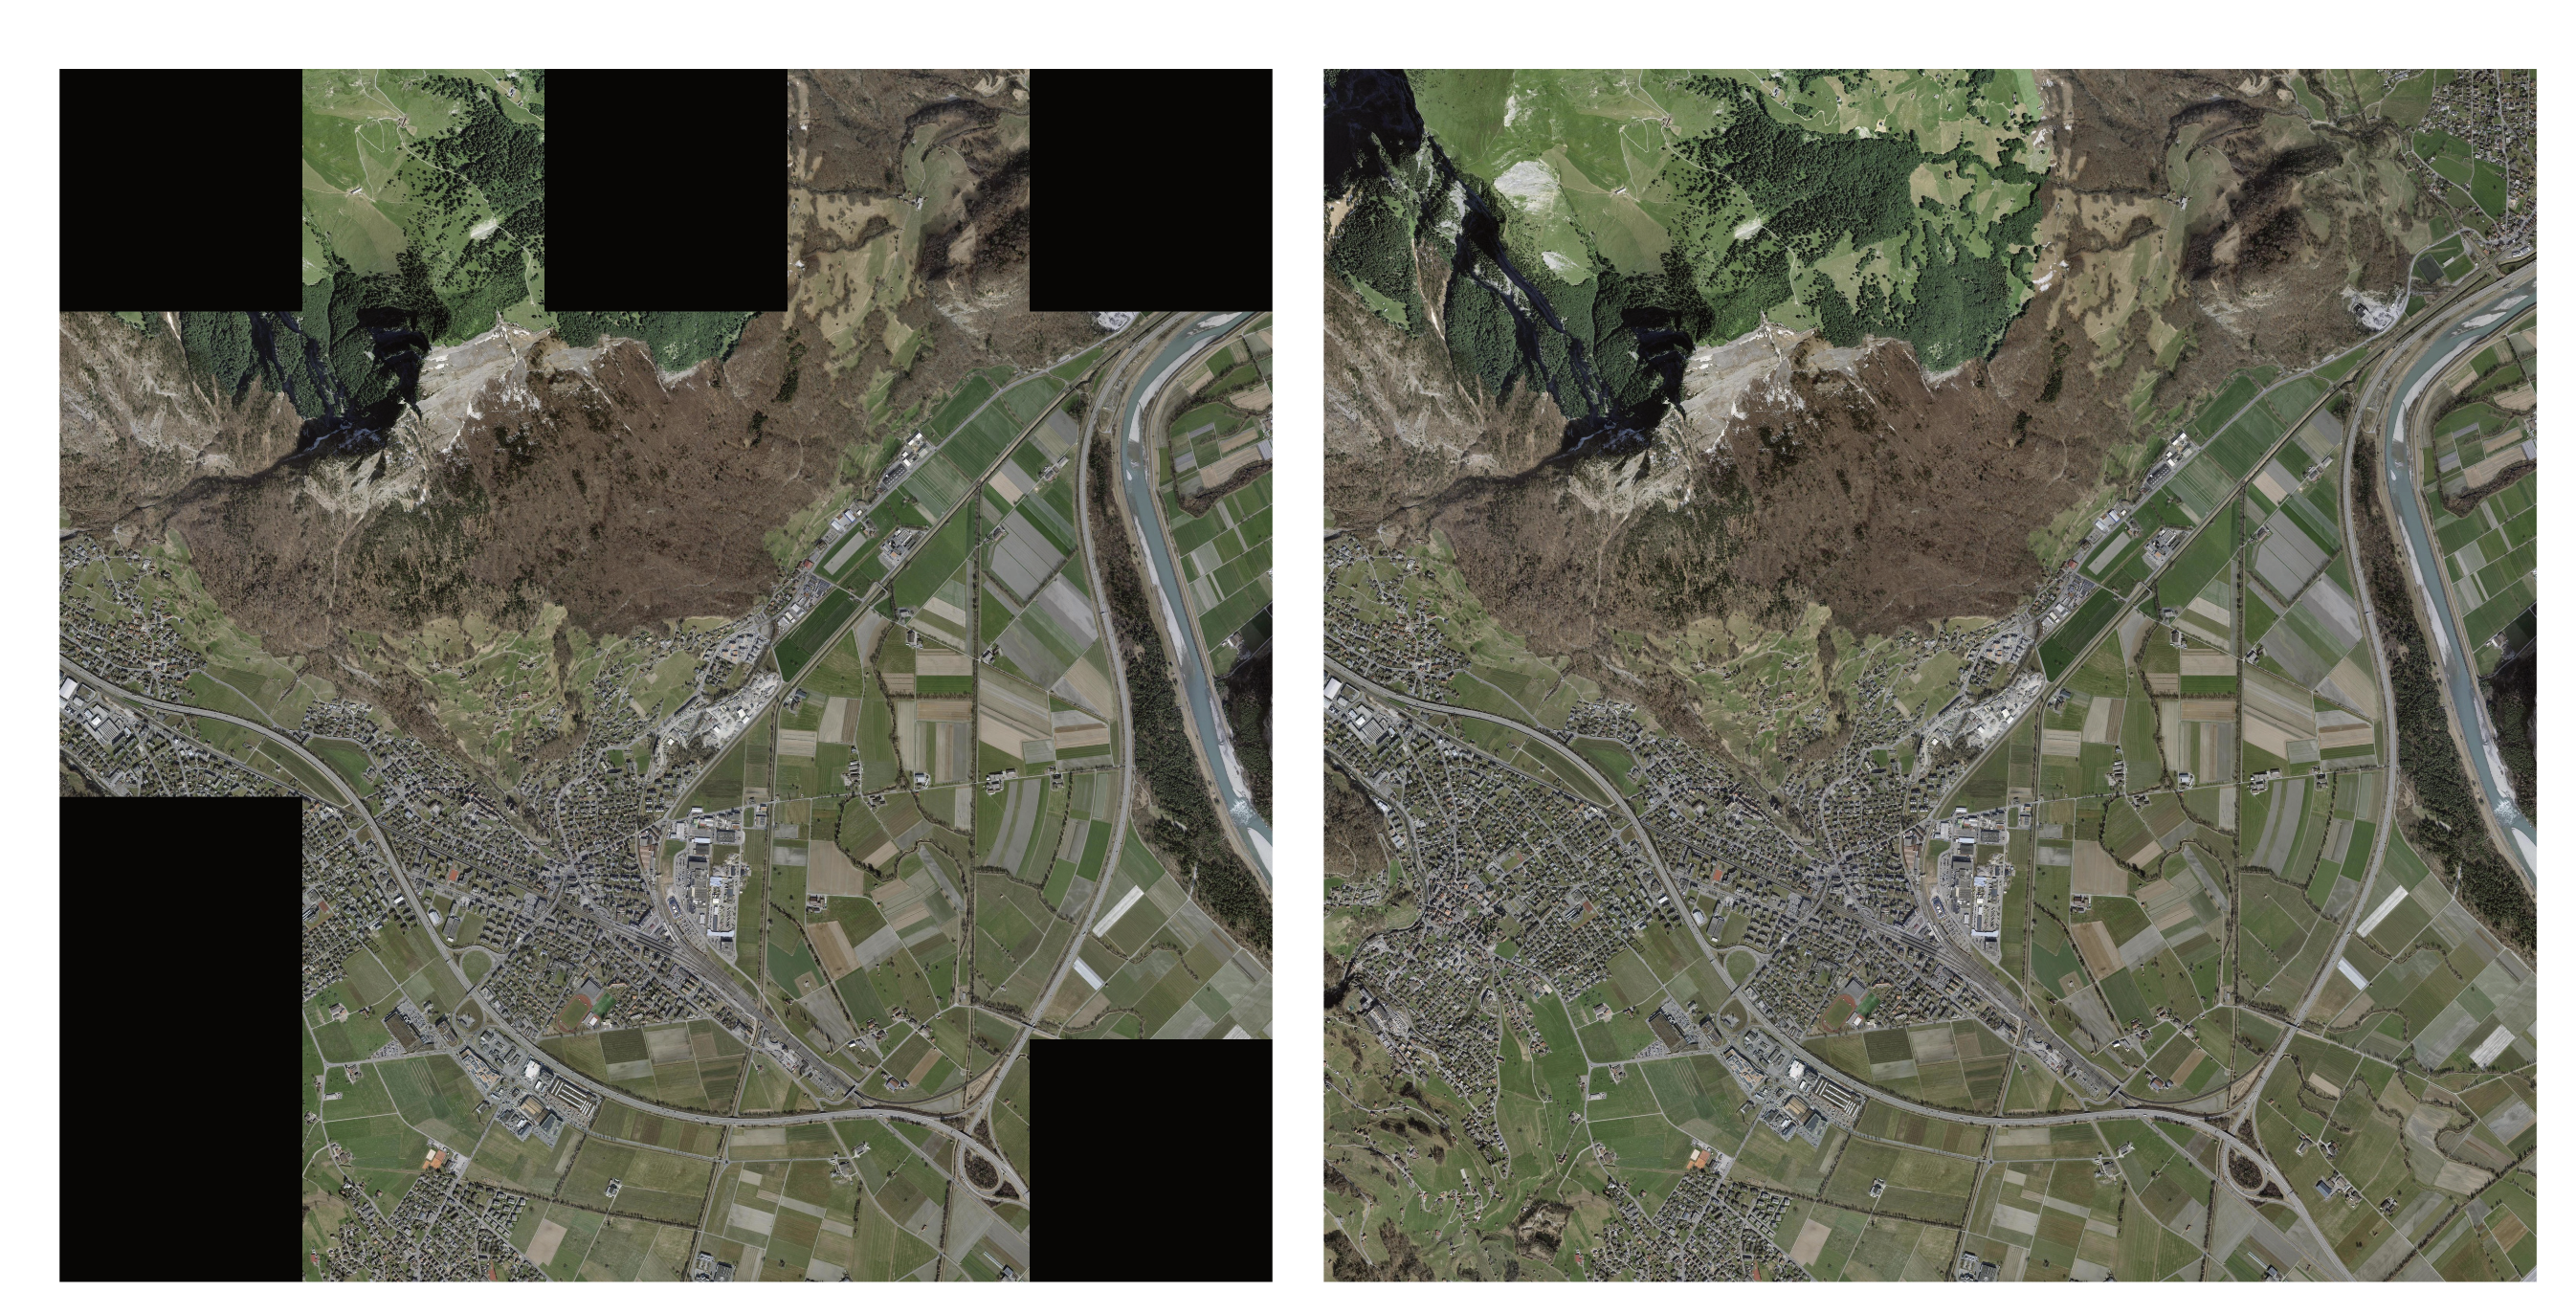
\includegraphics[width=.6\linewidth]{content/00_assets/gesamtbild_mit_luecken.png}
    \label{fig_swisstopo_daten_luecken}
\end{figure}

\subsection{Extrahierung der Höhenwerte und Bilddaten}
Nach dem Herunterladen der Daten werden sowohl die Bild- als auch die Höheninformationen aus den GeoTIFF-Dateien extrahiert und als eigenständige Texturen gespeichert. Die Höhenwerte liegen dabei in Form eines Graustufenbildes vor. Weiss repräsentiert hohe Werte, wohingegen niedrige Werte mit der Farbe Schwarz visualisiert sind (siehe Abbildung \ref{fig_heightmap_beispiel}). 
\begin{figure}[H]
    \caption{Extrahierte Höhenwerte als Graustufenbild (Eigene Darstellung)}
    \includegraphics[width=.4\linewidth]{content/00_assets/heightmap_beispiel.png}
    \label{fig_heightmap_beispiel}
\end{figure}

Um die Geopositionsdaten nicht zu verlieren, werden diese in den Dateinamen geschrieben. Da die Daten von swisstopo in Form von Tiles zur Verfügung gestellt werden, müssen diese in einem nächsten Schritt zu einem Gesamtbild zusammengesetzt werden. Da die Geoposition anhand des LV95-Koordinatensystems bekannt ist, können diese mittels der Nord- und Ostachsenwerte entsprechend zusammengesetzt werden. Hierbei zeigt sich jedoch ein Problem. Jede Kachel besitzt einen eigenen minimalen sowie maximalen Höhenwert. Werden diese zusammengesetzt, so gibt es keine fliessenden Übergänge. Um dieses Problem zu lösen, wurden die Höhenwerte mithilfe des globalen Minimums und Maximums normalisiert (siehe Abbildung \ref{fig_heightmap_sargans}).
\begin{figure}[H]
    \caption{Zusammengesetztes Graustufenbild von Sargans mit fliessenden (links) und nicht fliessenden (rechts) Übergängen (Eigene Darstellung)}
    \includegraphics[width=.7\linewidth]{content/00_assets/heightmap_sargans.png}
    \label{fig_heightmap_sargans}
\end{figure}

Das Extrahieren der Farbwerte aus dem swissIMAGE-Datensatz ist einfacher, da lediglich die Farbwerte aus den Dateien herausgelesen werden müssen und keine Normalisierung notwendig ist (siehe Abbildung \ref{fig_textur_sargans}). Aufgrund unterschiedlicher Aufnahmezeiträume können jedoch visuelle Diskrepanzen wie im Bereich A (siehe Abbildung \ref{fig_textur_sargans}) entstehen.
\begin{figure}[H]
    \caption{Zusammengesetztes Luftbild von Sargans (Eigene Darstellung)}
    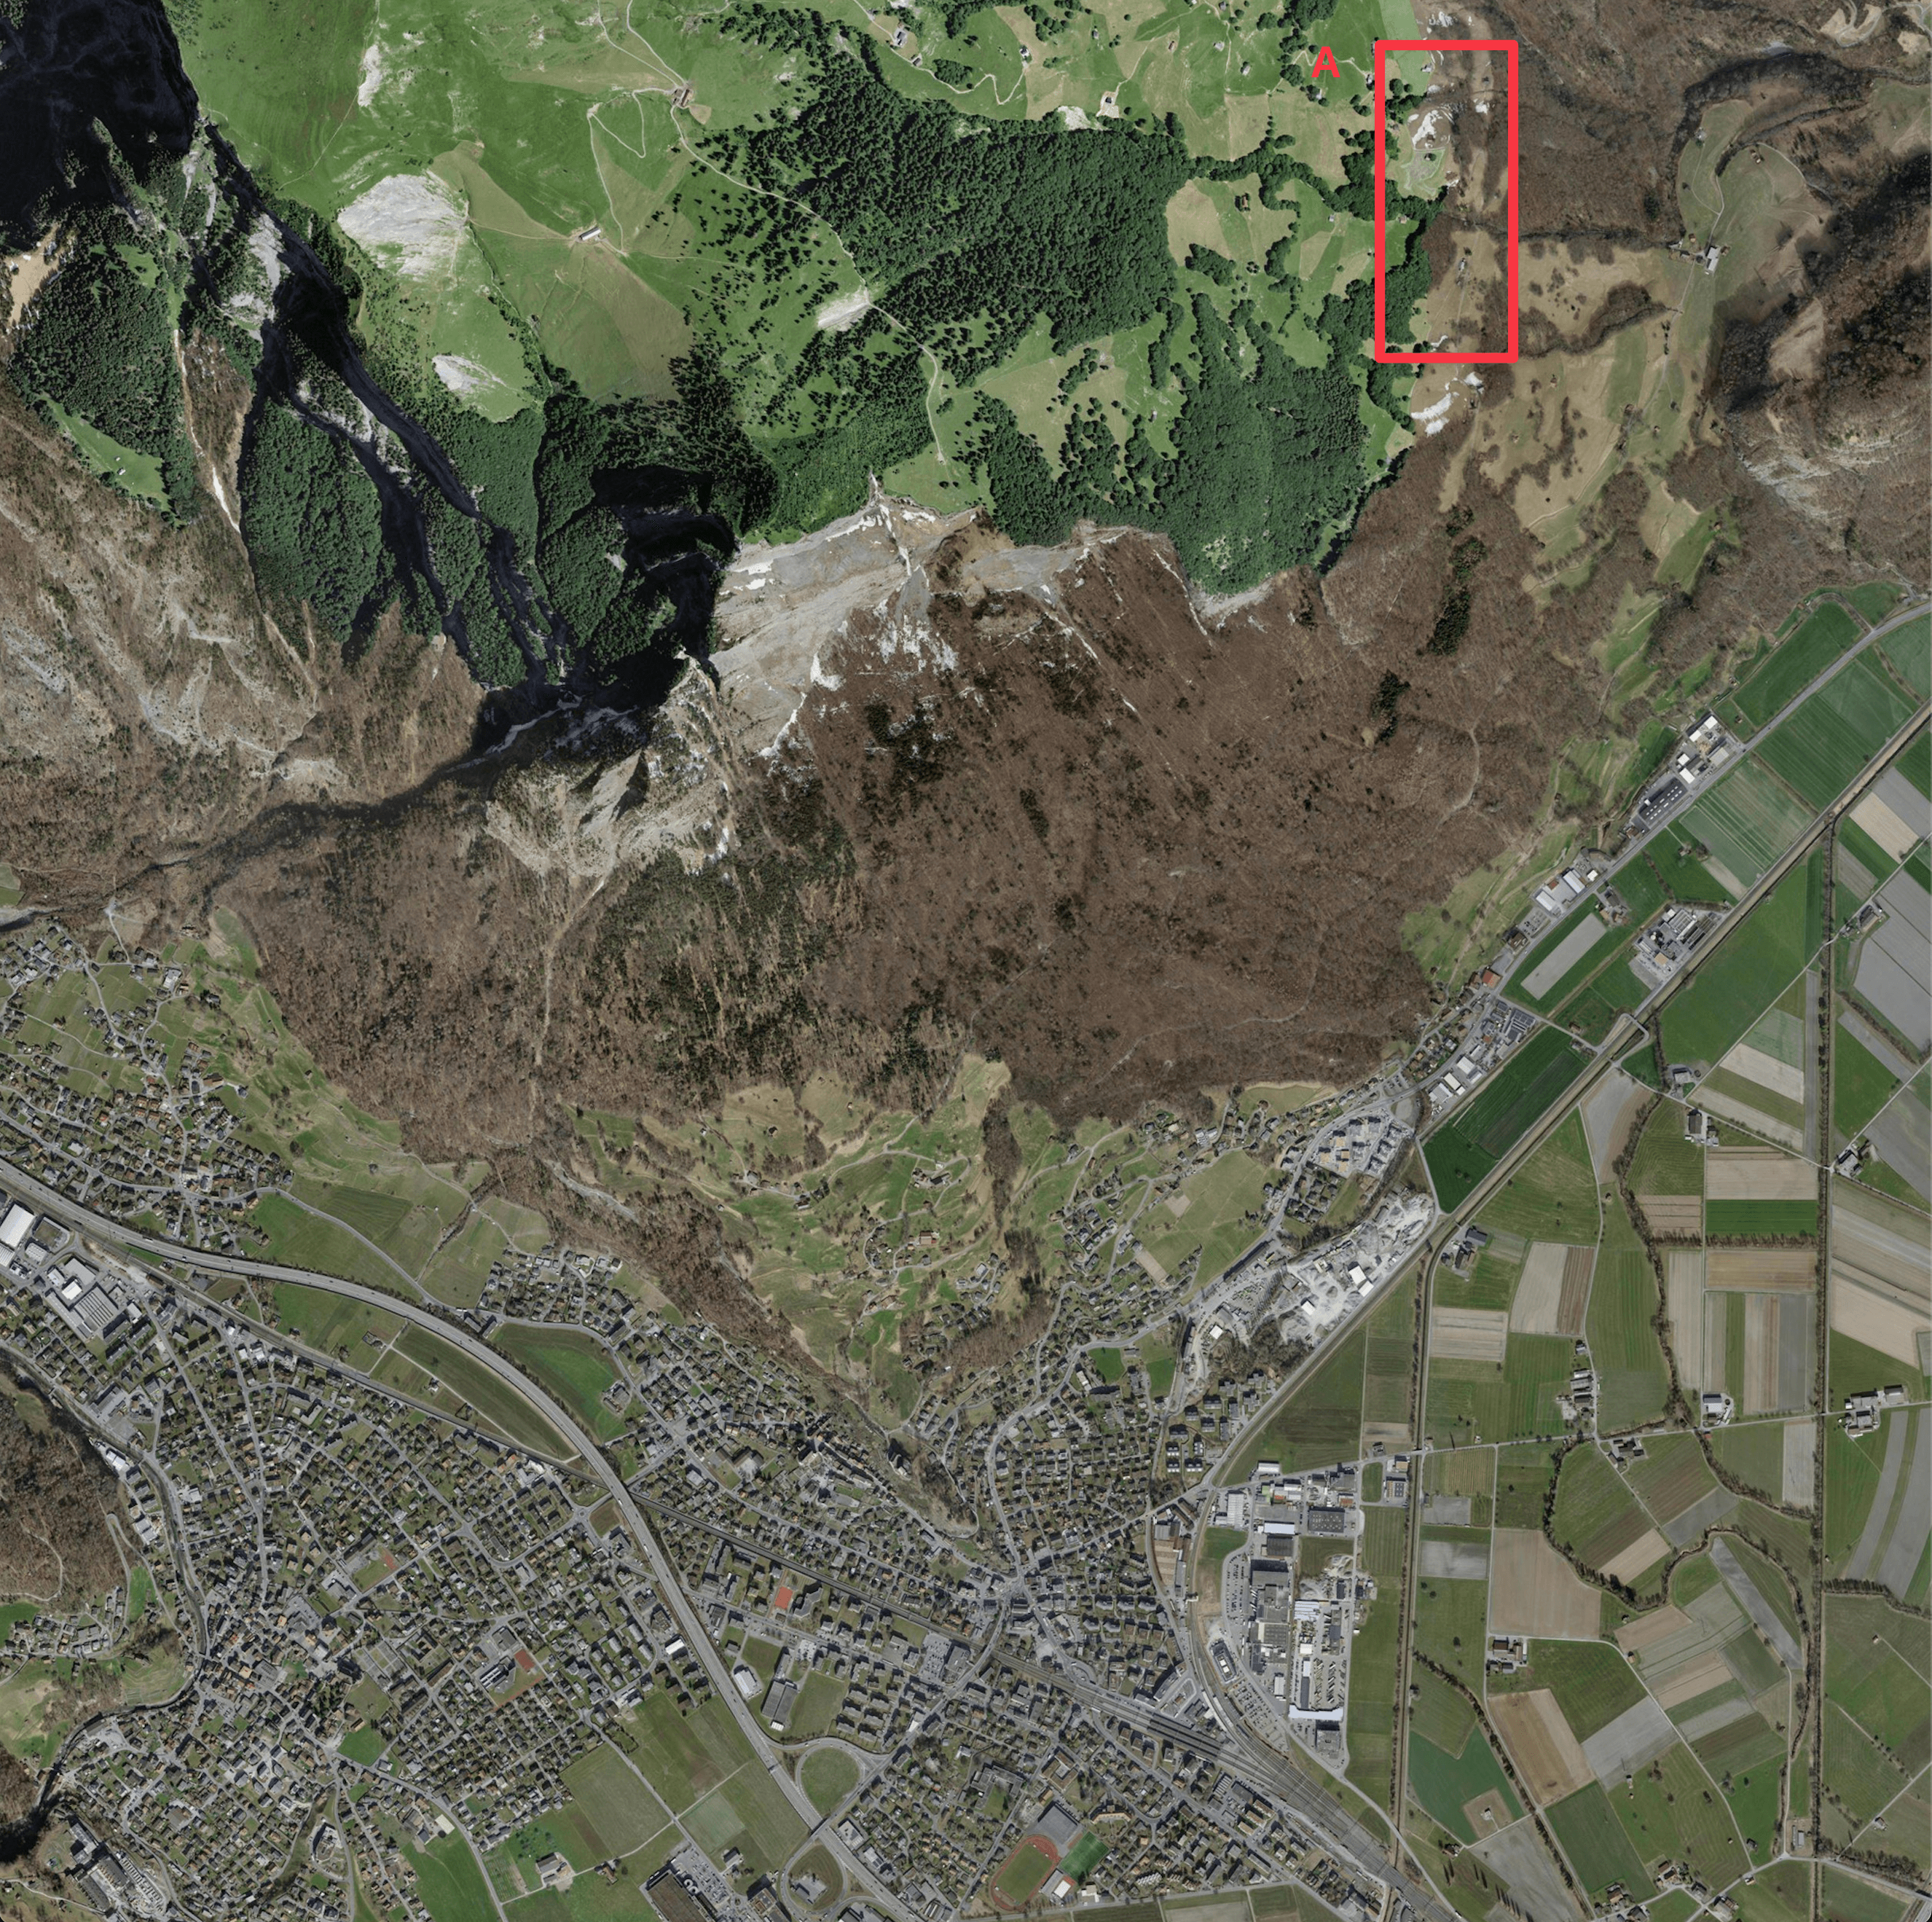
\includegraphics[width=.4\linewidth]{content/00_assets/textur_sargans.png}
    \label{fig_textur_sargans}
\end{figure}

\subsection{Aufteilung in kleinere Bilddateien}
Wie in Kapitel \ref{chap_datengrundlage} beschrieben, variiert der benötigte Festplattenspeicher der swisstopo-Datensätze abhängig von Auflösung und Gebiet. Für die Region Sargans ergibt sich bei der höchsten Auflösung von 10cm pro Bildpunkt ein zusammengesetztes Luftbild mit einer Grösse von rund  7.5GB. Eine derart grosse Datenmenge ist für eine browserbasierte Anwendung nur bedingt geeignet, da andernfalls lange Ladezeiten auftreten würden. Browserbasierte Anwendungen haben gegenüber nativen Applikationen zwar den Vorteil, dass sie von überall aus zugreifbar sind, jedoch müssen hierzu die notwendigen Daten auch auf das Zielsystem des Nutzers heruntergeladen werden. Je nach Internetbandbreite kann dieser Prozess viel Zeit benötigen. Das Herunterladen von grossen Dateien ist daher trotz Konzepten wie Ladebalken keine skalierbare Lösung.

Zur Lösung dieses Problems werden im Rahmen der Datenvorverarbeitung mehrere Verarbeitungsschritte durchgeführt. Zunächst wird das Gesamtbild in kleinere Bilddateien, sogenannte Tiles, unterteilt. Um den Speicherbedarf zu reduzieren und die Ladezeiten zu verkürzen, werden diese Tiles anschliessend mithilfe eines Downsampling-Algorithmus skaliert.


Die Aufteilung der Bilddaten erfolgt auf Basis eines Quadtree-Algorithmus, wobei Tiles in unterschiedlichen Auflösungsstufen (Level of Detail, LOD) erzeugt werden. Die jeweilige Auflösung ist dabei direkt an die Baumtiefe des Quadtrees gekoppelt. Für die erste Auflösung (LOD 1) wird das Gesamtbild in 4 (4$^1$) Tiles aufgeteilt. Für die zweite Auflösung sind es hingegen 16 (4$^2$) und so weiter. Abbildung \ref{fig_textur_teilbilder_quadtree} veranschaulicht die Aufteilung eines Gesamtbildes in Tiles unterschiedlicher Auflösung.
\begin{figure}[H]
    \caption{Aufteilung in Tiles mit unterschiedlichen Auflösungen (Eigene Darstellung)}
    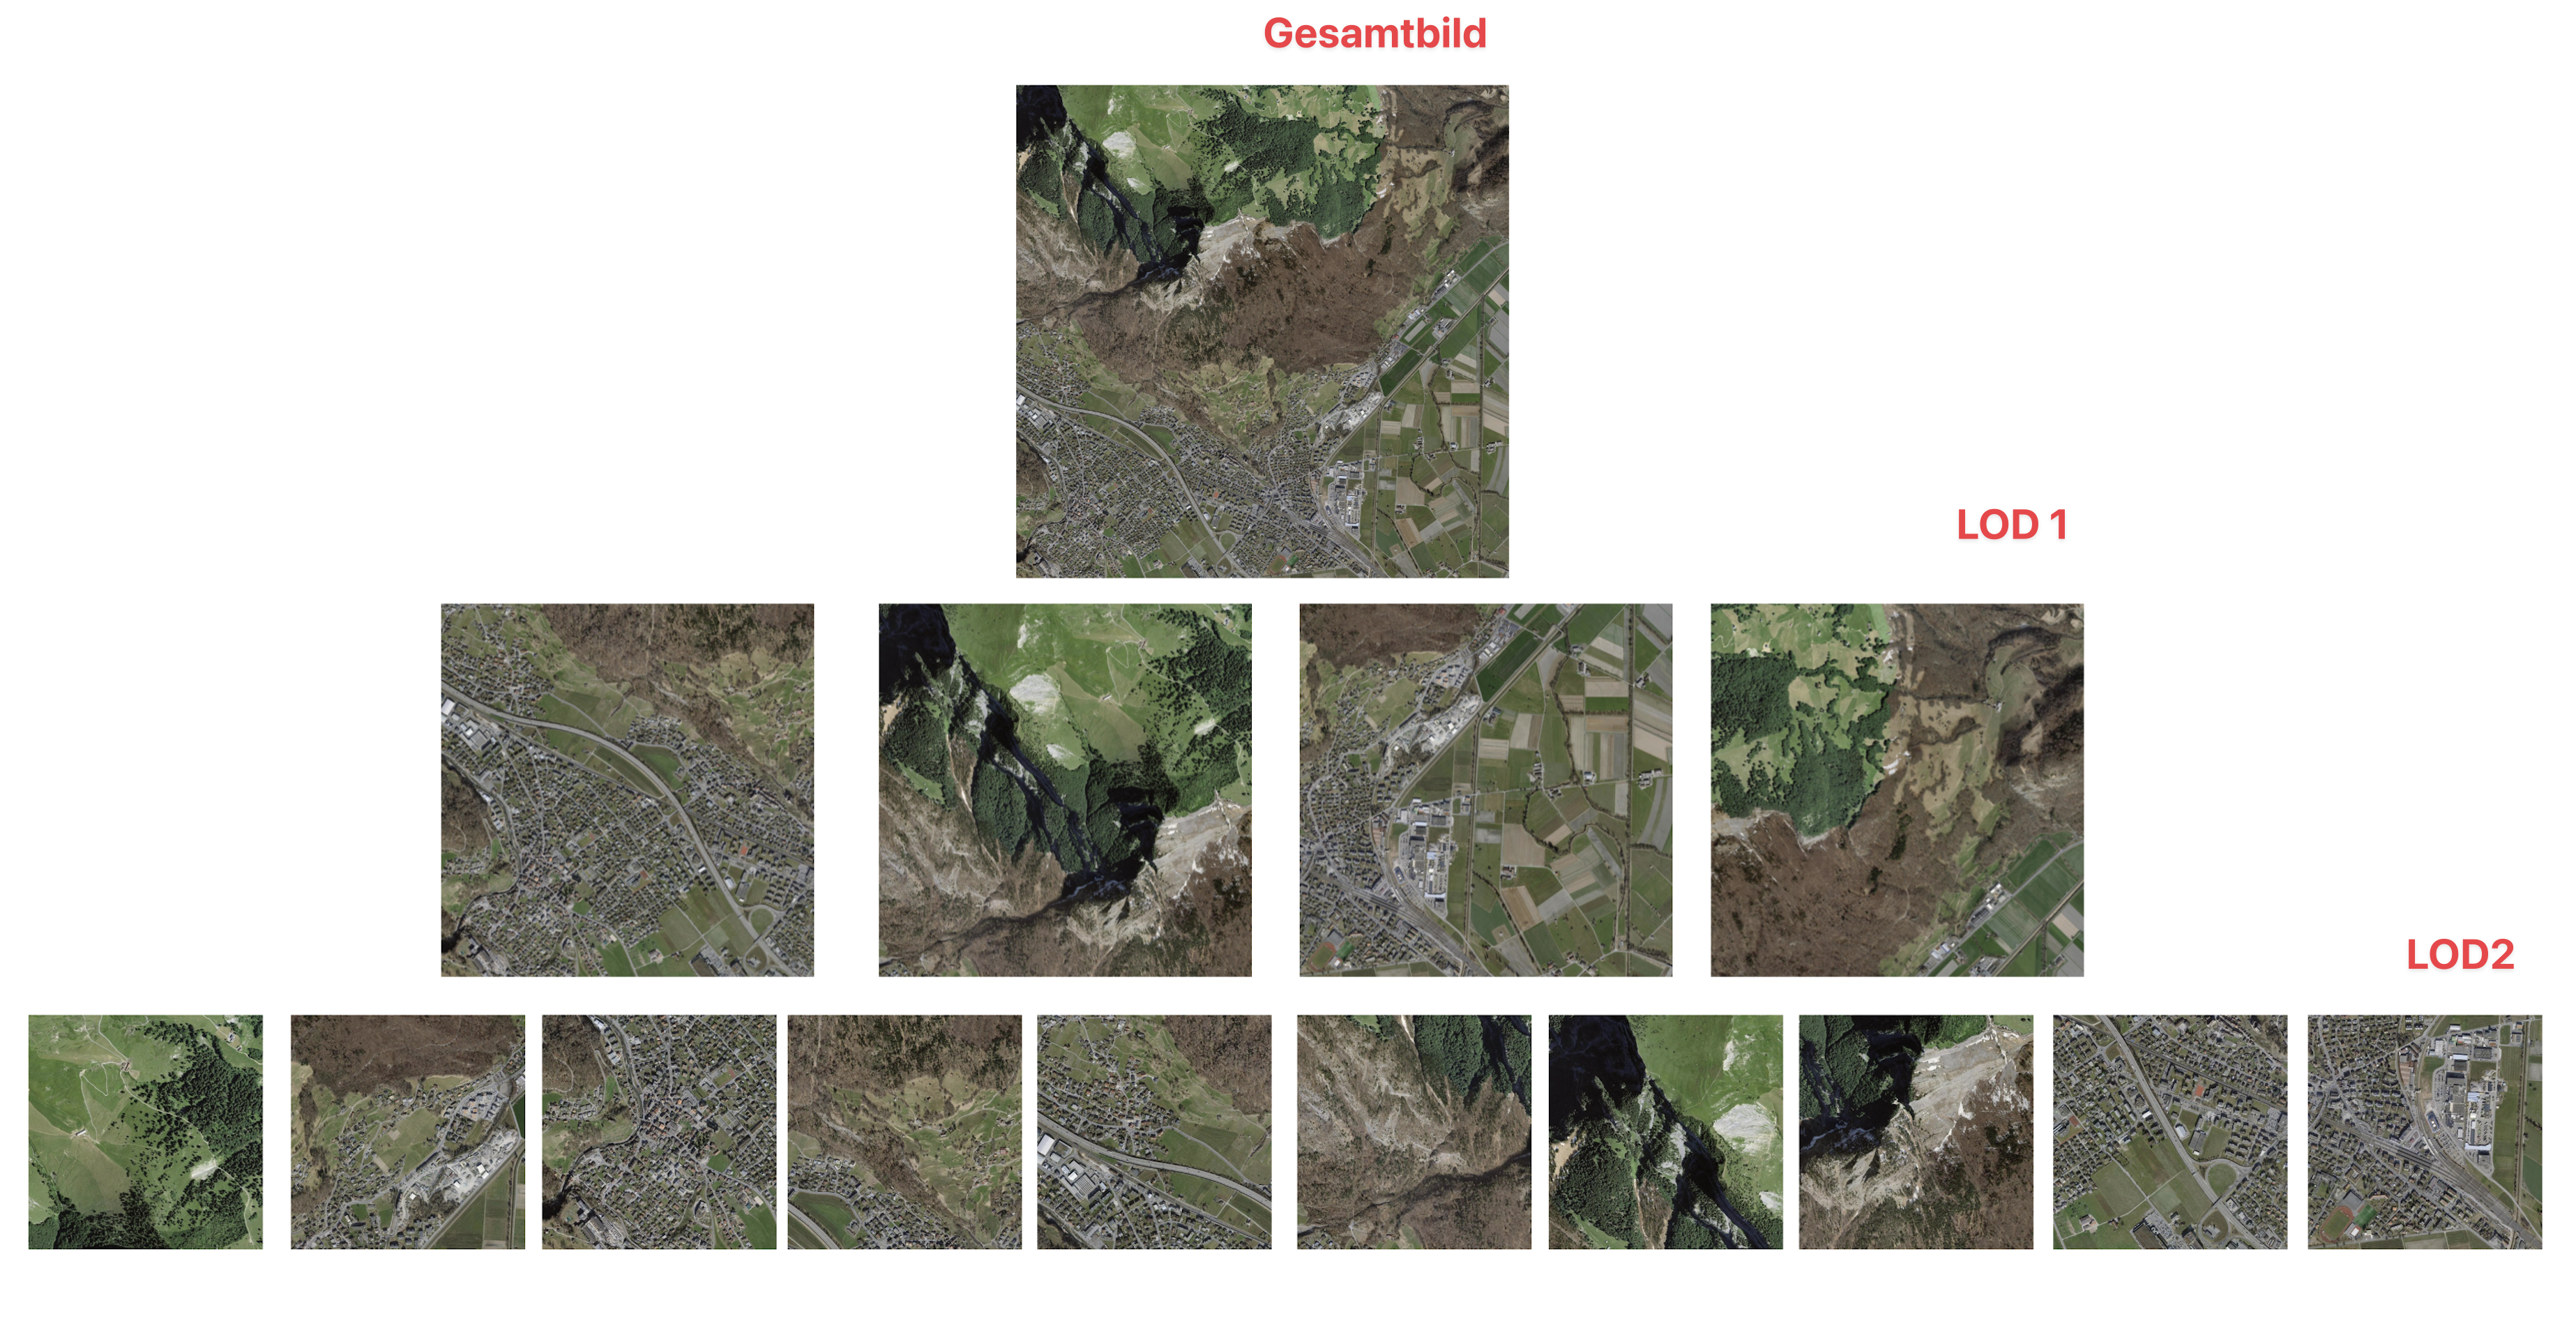
\includegraphics[width=1.0\linewidth]{content/00_assets/zerlegung_in_teilbilder.png}
    \label{fig_textur_teilbilder_quadtree}
\end{figure}

\subsection{Ermittlung des quadratischen Bildausschnitts}
Grafikkarten bevorzugen Texturen mit gleich langen Seiten (bspw. 500 x 500 Pixel). Das Gesamtbild weist je nach Region und Ausschnitt jedoch unterschiedliche Seitenverhältnisse auf. Daher wird dieses zusätzlich auf einen quadratischen Bereich eingeschränkt (siehe Abbildung \ref{fig_begrenzung_bildausschnitt}). Der quadratische Ausschnitt wird hierbei so gewählt, dass das Gesamtbild restlos durch Tiles in der höchsten Auflösung (LOD 2 in Abbildung \ref{fig_textur_teilbilder_quadtree}) aufgeteilt werden kann.
\begin{figure}[H]
    \caption{Begrenzung Bildausschnitt (Eigene Darstellung)}
    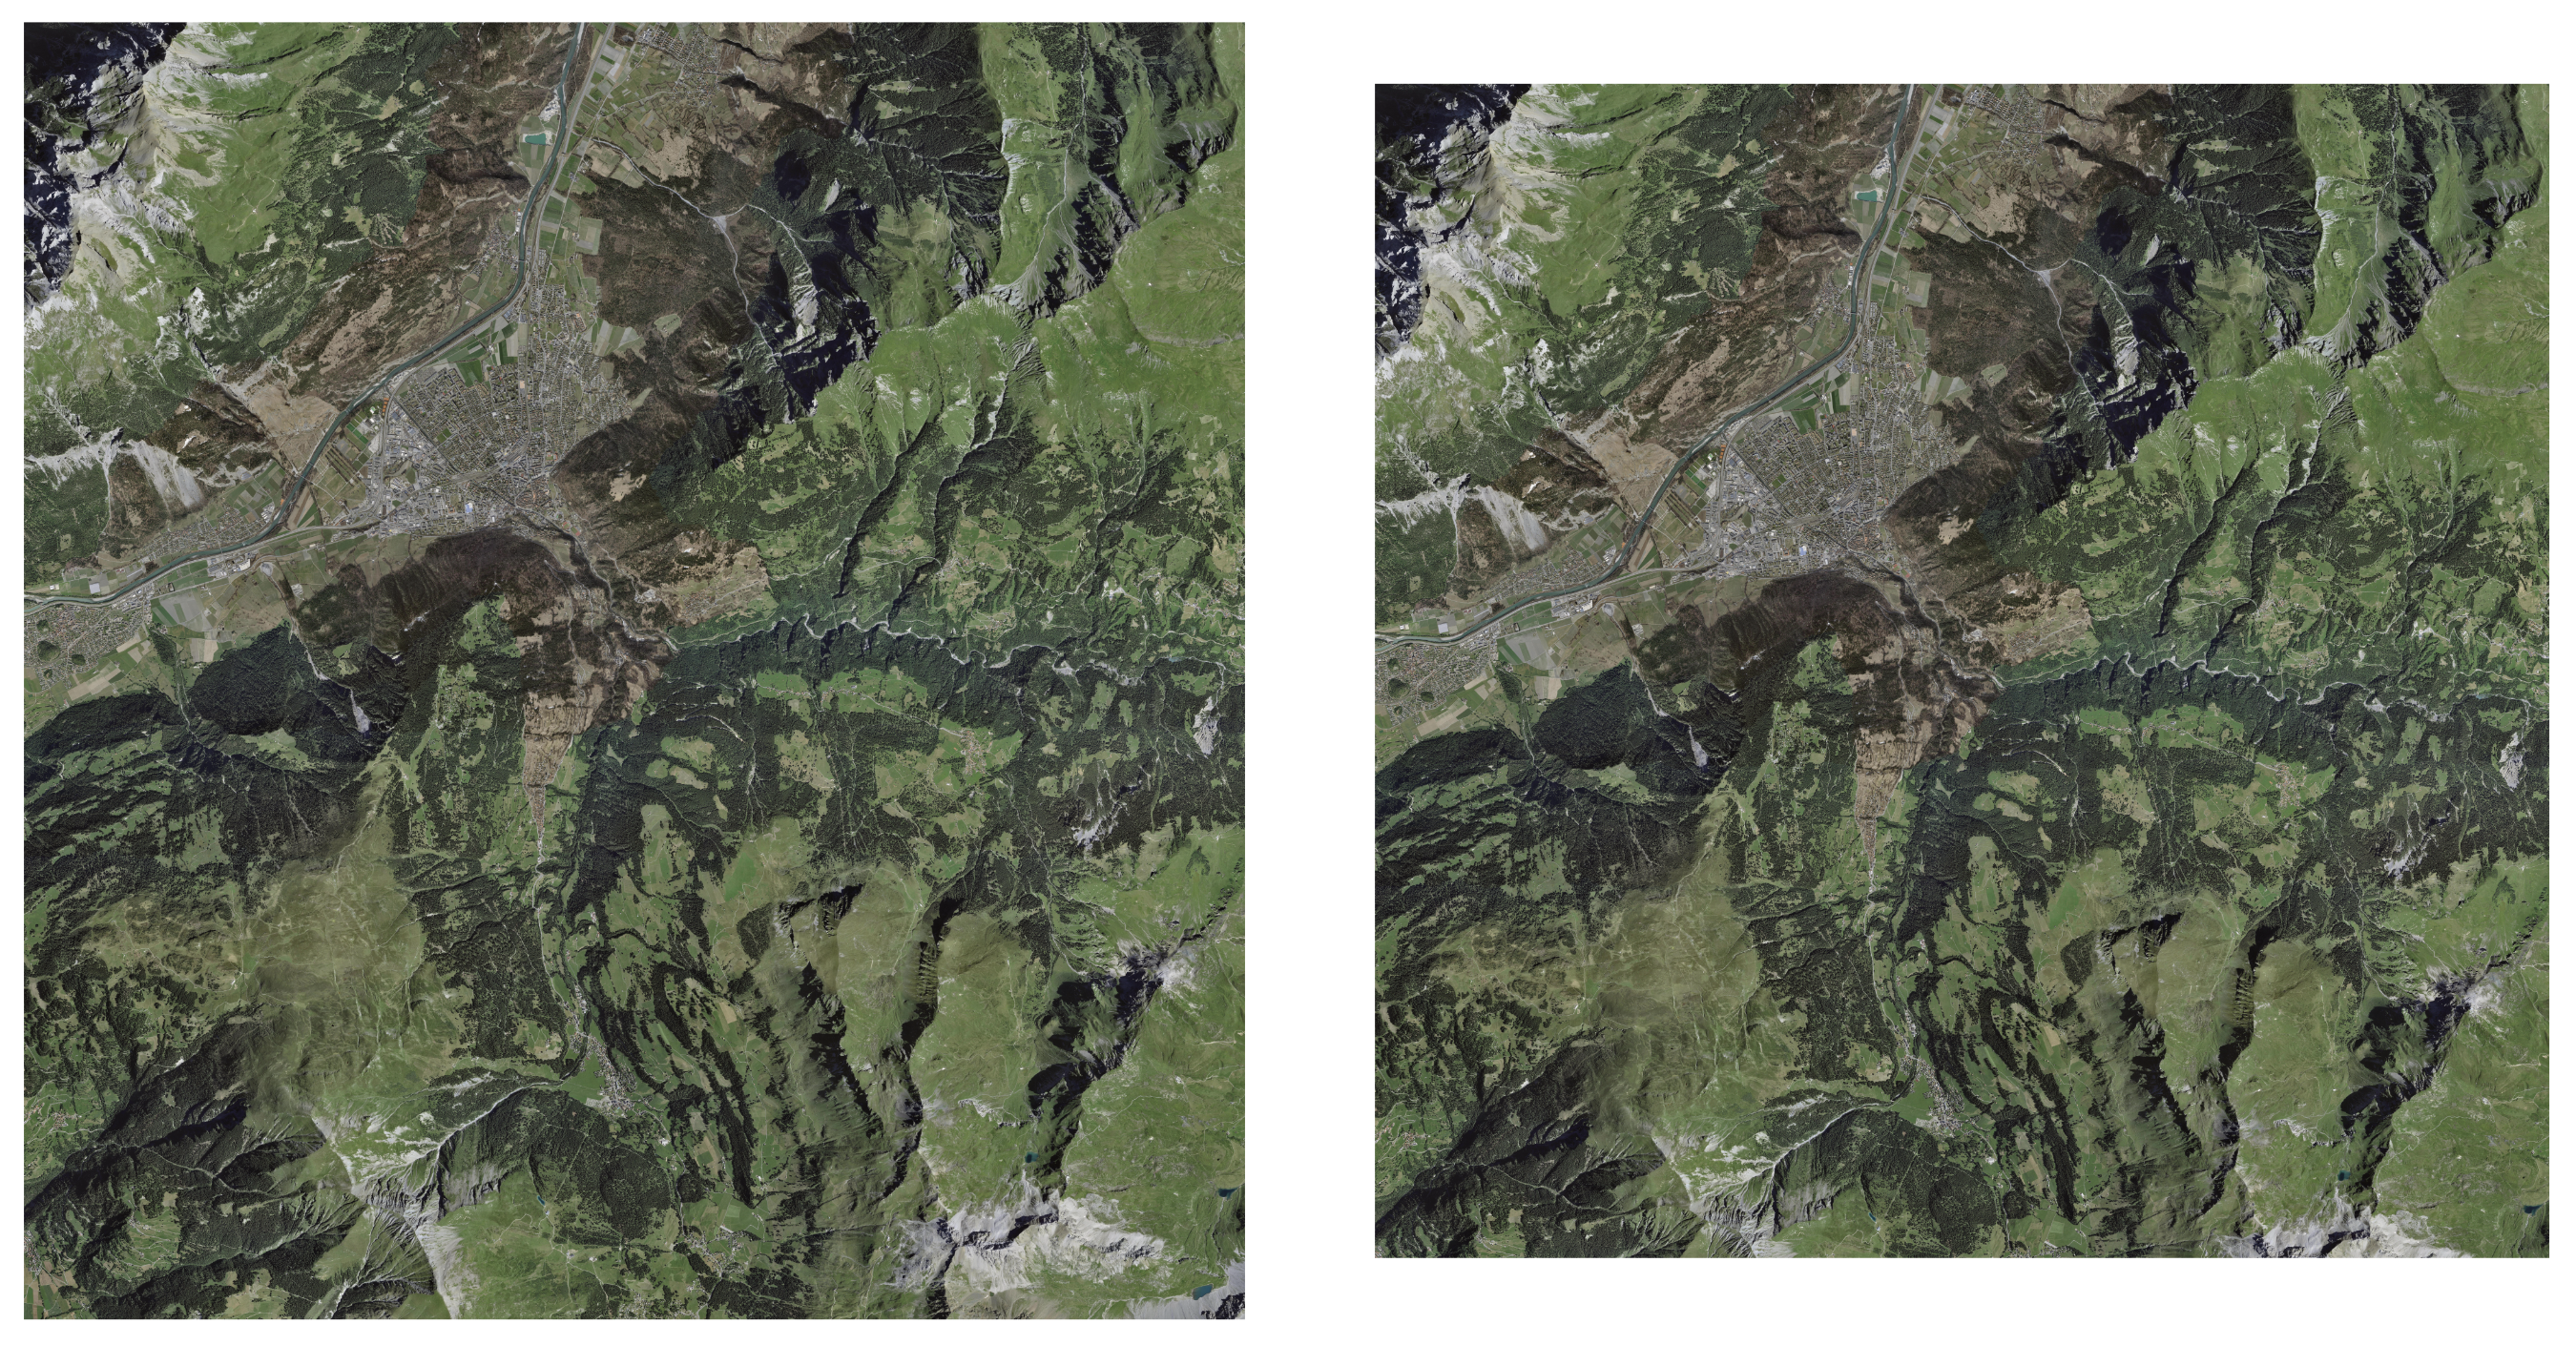
\includegraphics[width=.7\linewidth]{content/00_assets/begrenzung_bildausschnitt.png}
    \label{fig_begrenzung_bildausschnitt}
\end{figure}

\subsection{Automatische Ermittlung der maximalen Baumtiefe}
\label{chap_ermittlung_baumtiefe}
Da sich die Erstellung der Tiles am Quadtree Algorithmus orientiert, lassen sich die maximale Baumtiefe und somit die höchste verfügbare Detailstufe bereits im Vorfeld bestimmen. Zur Veranschaulichung dient folgendes Beispiel: Das Luftbild der Region Sargans weisst eine Auflösung ($R$) von 2000 auf 2000 Bildpunkten auf. Bei einer Bodenauflösung von 2m pro Bildpunkt ergibt sich daraus eine effektive Tile-Auflösung ($T$) von 500px ($\frac{1000m}{\frac{2m}{1px}}$) pro km$^2$. Die maximale Baumtiefe ($L_{\max}$) kann auf Basis dieser Parameter mithilfe der Logarithmusfunktion berechnet werden. Für die Region Sargans ergibt sich daraus eine maximale Baumtiefe von 3, was der höchsten darstellbaren Detailstufe entspricht.
\[
L_{\max} = (\log_2\frac{R}{T}) + 1
\]

\subsection{Border Patching}
Auf Basis der extrahierten Höhen- und Bildinformationen lassen sich 3D-Modelle rekonstruieren. Die konkrete Generierung der Geometrie wird in Kapitel \ref{chap_erstellung_geometrie} beschrieben. Werden mehrere dieser Modelle nebeneinander angeordnet, zeigen sich an den Übergängen zwischen benachbarten Tiles sichtbare Risse (siehe schwarze Bereiche in Abbildung \ref{fig_risse_zwischen_3d_modellen}). Diese Artefakte entstehen, da die Höhenwerte entlang der gemeinsamen Kanten nicht exakt mit den Höhenwerten der angrenzenden Tiles übereinstimmen. Infolgedessen weichen die Positionen der entsprechenden Vertices voneinander ab, wodurch sichtbare Lücken in der Geometrie entstehen.
\begin{figure}[H]
    \caption{Risse zwischen 3D Modellen der gleichen Detailstufe (Eigene Darstellung)}
    \includegraphics[width=.3\linewidth]{content/00_assets/risse_zwischen_gleichen_detailstufen.png}
    \label{fig_risse_zwischen_3d_modellen}
\end{figure}

Diese Problematik kann mit dem sogenannten ``Border Patching'' eliminiert werden. Hierzu werden an den Schnittkanten die Daten der angrenzenden Nachbarn übernommen und so ein Überlappungsbereich geschaffen. Bereits ein Bereich von einem Pixel reicht aus, um die Risse zu eliminieren. Abbildung \ref{fig_border_patching} stellt den Überlappungsbereich in Form von roten Linien dar. An diesen Kanten werden jeweils die Werte der Nachbarn (d.h. von 1 nach 2 etc.) übernommen.
\begin{figure}[H]
    \caption{Border Patching (Eigene Darstellung)}
    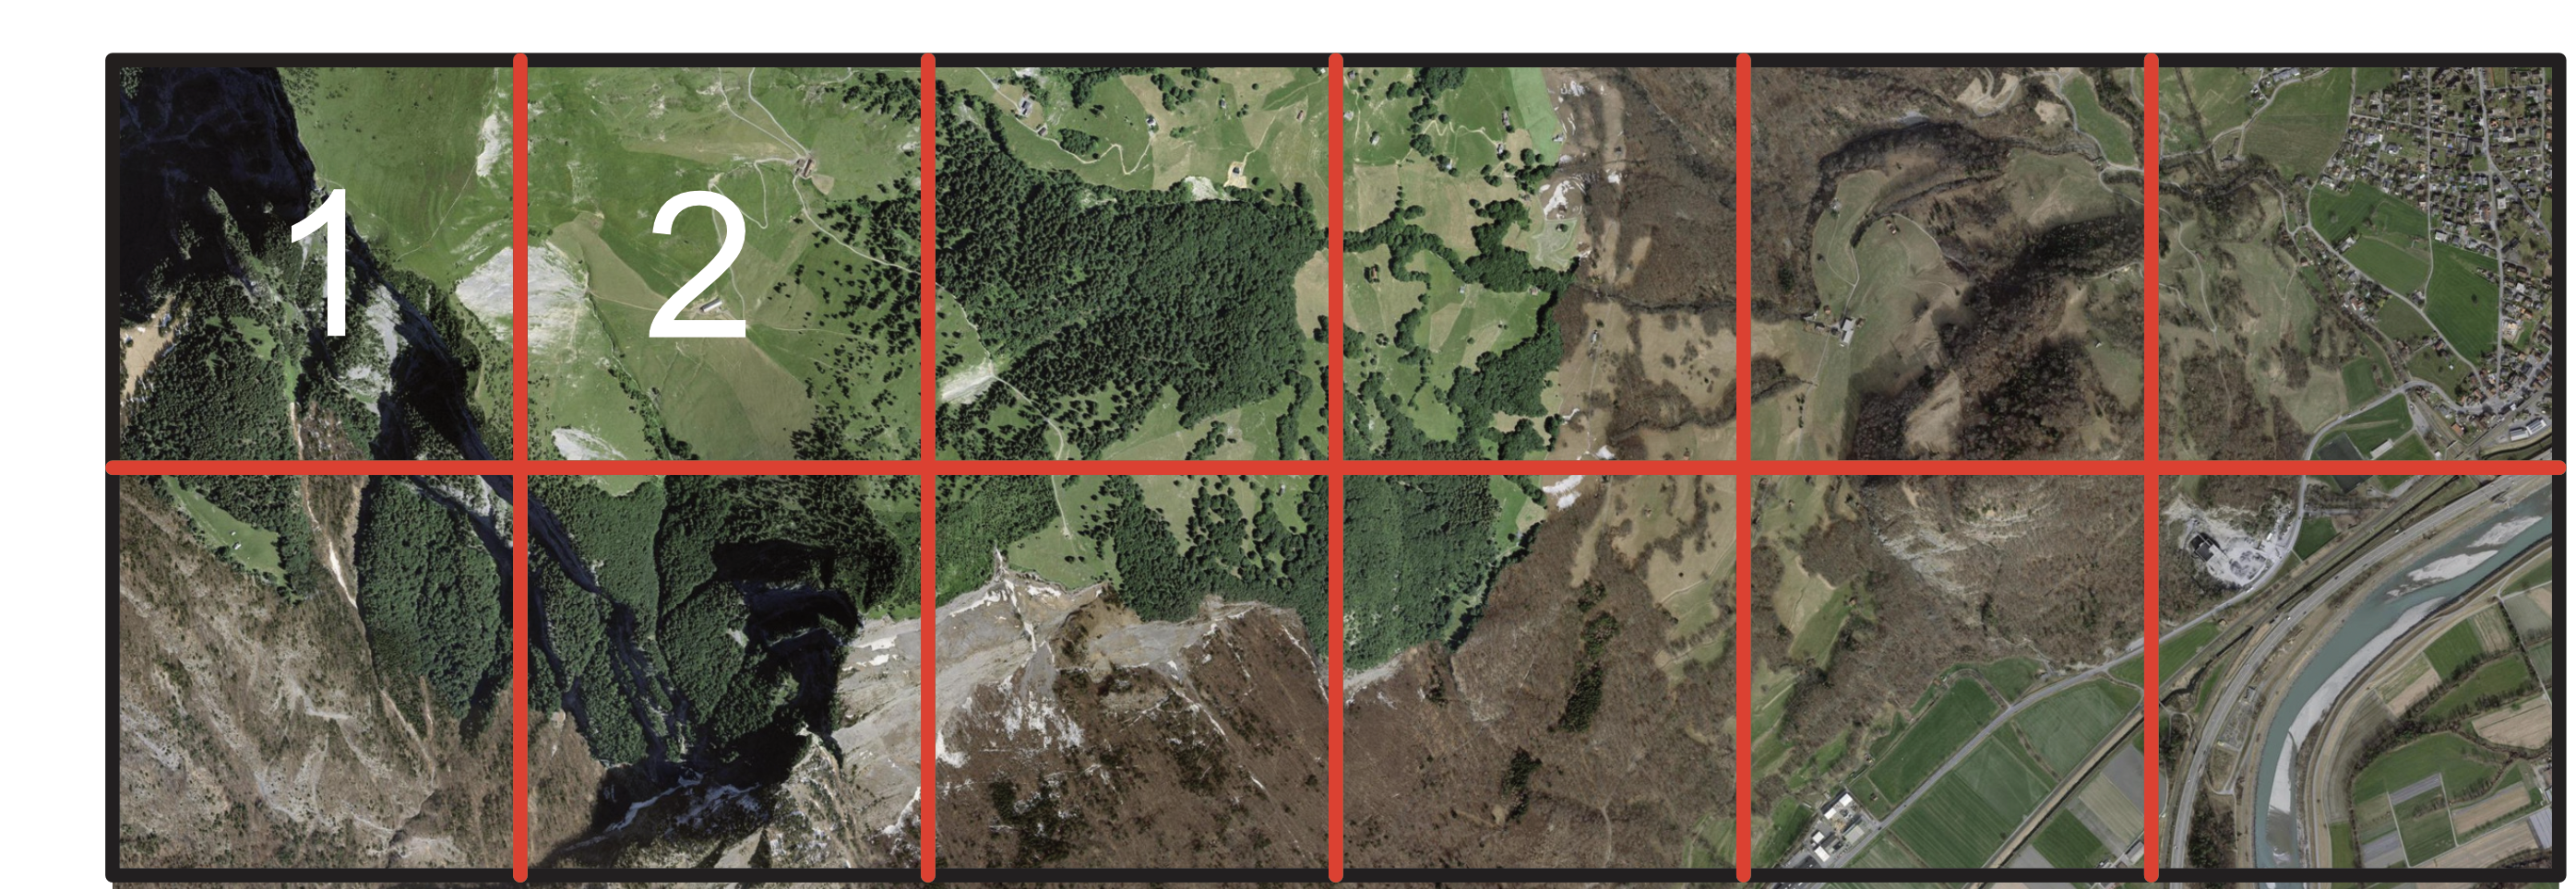
\includegraphics[width=.5\linewidth]{content/00_assets/border_patching.png}
    \label{fig_border_patching}
\end{figure}

\subsection{Relative Geopositionsinformationen}
Das Three.js Koordinatensystem weist einen anderen Koordinatenmittelpunkt (0/0) auf als die swisstopo Daten (2'600'000/1'200'000). Um die 3D-Modelle korrekt in Three.js zu positionieren werden relative Geopositionsinformationen berechnet. Dafür wird zuerst der Mittelpunkt des Gesamtbildes im LV95 Koordinatensystem bestimmt. Anschliessend wird für jede Tile der relative Abstand zu diesem Mittelpunkt ermittelt und in den Metadaten abgespeichert. Somit ist sichergestellt, dass die 3D-Modelle relativ um den Three.js Koordinatenmittelpunkt platziert werden können.

\subsection{Generierung von Metadaten}
\label{chap_generierung_metadaten}
Um wichtige Informationen in Bezug auf die swisstopo Daten nicht zu verlieren werden entsprechende Metadaten generiert. Die Metadaten werden als JSON-Datei (siehe Abbildung \ref{fig_ausschnitt_metadaten}) abgespeichert und entsprechend zur Laufzeit der Webanwendung eingelesen. Tabelle \ref{table_metadata} gibt einen Überblick über die Metadaten sowie den Verwendungszweck.
\begin{table}[H]
    \caption{Erstellte Metadaten und Verwendungszweck (Eigene Darstellung)}
    \begin{tabularx}{\textwidth} {
        >{\raggedright\arraybackslash}X 
        >{\raggedright\arraybackslash}X}
            \hline
            \textbf{Metadaten} & {Verwendungszweck}  \\
            \hline
            Absolute Geopositionsinformationen (LV95) & LV95 Koordinaten der Tiles \\
            Relative Geopositionsinformationen (LV95) & Relative Positionierung der Tiles zum Three.js Koordinatenmittelpunkt \\
            Maximale Baumtiefe & Limitierungskriterium für den Quadtree Algorithmus \\
            Dateipfade zu den erstellten Bilddateien & Werden zur Laufzeit geladen und bilden die Grundlage für die 3D-Geometrien \\
            \hline
    \end{tabularx}
    \bigbreak
    \label{table_metadata}
\end{table}

\begin{figure}[H]
    \caption{Auszug aus den generierten Metadaten (Eigene Darstellung)}
    \includegraphics[width=.5\linewidth]{content/00_assets/ausschnitt_metadaten.png}
    \label{fig_ausschnitt_metadaten}
\end{figure}

\section{Implementierung}
Dieses Kapitel widmet sich der eigentlichen Implementierung der 3D-Terrainvisualisierung auf Basis des Three.js Frameworks und der swisstopo-Daten. Zu Beginn wird die Erstellung der eigentlichen 3D-Modelle anhand der vorverarbeiteten Daten erläutert. Anschliessend werden die eingesetzten Algorithmen sowie entsprechende Hilfsvisualisierungen thematisiert. Abgerundet wird dieses Kapitel mit der Implementierung der Steuerungselemente zur freien Bewegung im 3D-Raum. Die Terrainvisualisierung steht unter der MIT-Lizenz und ist auf GitHub\footnote{\url{https://github.com/yhutter/swiss-terrain-3d}} verfügbar.

\subsection{Erstellung der 3D-Geometrie}
\label{chap_erstellung_geometrie}
Um das Gebirge in 3D zu visualisieren wird für die Geometrie ein Gitternetz von Punkten eingesetzt. In Three.js wird hierfür die sogenannte ``PlaneGeometry'', welche eine Ebene im 3D-Raum darstellt, verwendet (siehe Abbildung \ref{fig_threejs_plane_geometry}). Die Auflösung dieser Geometrie kann beliebig verfeinert werden, wodurch schlussendlich ein Gitternetz entsteht.
\begin{figure}[H]
    \caption{Three.js PlaneGeometry \parencite{threejs_beispiel_plane_geometry_2025}}
    \includegraphics[width=.3\linewidth]{content/00_assets/threejs_plane_geometry.png}
    \label{fig_threejs_plane_geometry}
\end{figure}

Um Risse im Terrain zwischen verschiedenen LOD's zu vermeiden wird anstelle eines diagonalen ein sternförmiges Muster (siehe Abbildung \ref{fig_plane_geometry_star_structure}) verwendet. In Kombination mit dem sogenannten ``Index-Stitching'' lassen sich hiermit Risse eliminieren (die genaue Erläuterung folgt in Kapitel \ref{chap_quadtree_algorithmus}). 
\begin{figure}[H]
    \caption{Gitternetz mit sternförmiger Struktur \parencite[S. 54]{frostbite_terrain_rendering_2007}}
    \includegraphics[width=.3\linewidth]{content/00_assets/geometry_star_pattern.png}
    \label{fig_plane_geometry_star_structure}
\end{figure}

Obwohl Three.js viele 3D-Geometrien zur Verfügung stellt, ist es ebenso möglich, eigene Geometrien zu definieren. Zu diesem Zweck stellt Three.js die Klasse \textit{BufferGeometry} zur Verfügung. Auf deren Basis wurde eine individuelle Geometrie erzeugt, um die gewünschte sternförmige Struktur abzubilden. Wie in Kapitel \ref{chap_render_pipelines} erläutert, setzen sich 3D-Modelle aus Dreiecken zusammen, die wiederum aus einzelnen Punkten, sogenannten Vertices, bestehen. Die Zusammensetzung dieser Punkte zu Dreiecken wird über sogenannte ``Indices'' definiert. Abbildung \ref{fig_create_geometry_with_indices} veranschaulicht diesen Prozess beispielhaft. Zur Erzeugung des Dreiecks $abi$ werden die Punkte $a$, $b$ und $i$ miteinander verbunden. Dieses Verfahren wird für alle weiteren Dreiecke wiederholt, bis die vollständige sternförmige Struktur entsteht. 
\begin{figure}[H]
    \caption{Erstellung der Geometrie mittels Indices (Eigene Darstellung)}
    \includegraphics[width=.7\linewidth]{content/00_assets/erstellung_geometry_mittels_indices.png}
    \label{fig_create_geometry_with_indices}
\end{figure}

Aktuell befinden sich alle Punkte auf einer Ebene. Um ein 3D-Modell zu erhalten, müssen die Punkte anhand der extrahierten Höhendaten entsprechend nach oben oder unten verschoben werden. Die Verschiebung der Punkte erfolgt im Vertex Shader (siehe Kapitel \ref{chap_render_pipelines}). Zuerst werden die Höhenwerte aus den Graustufenbildern gelesen und anhand des vorberechneten globalen Maximum- und Minimumhöhenwerts entsprechend skaliert. Die Vertices der Geometrie werden anschliessend anhand dieses Wertes entsprechend verschoben (siehe Abbildung \ref{fig_verschiebung_punkte_vertex_shader}). Der Code in Abbildung \ref{fig_verschiebung_punkte_vertex_shader} ist in einer Three.js spezifischen Programmiersprache für Shader mit dem Namen \acrfull{TSL} geschrieben. Wie in Kapitel \ref{chap_technologien} erläutert, unterstützt Three.js sowohl die WebGL als auch die neuere WebGPU Grafikschnittstelle. Die Programmiersprache dieser zwei Schnittstellen ist jedoch unterschiedlich. \acrshort{TSL} fungiert hier als ``Übersetzer'' zwischen diesen Sprachen und erlaubt es somit, beide Grafikschnittstellen mit derselben Programmiersprache anzusprechen. Three.js wählt selbständig je nach Hardwaresupport die geeignetste Grafikschnittstelle aus. 
\begin{figure}[H]
    \caption{Verschiebung der Punkte im Vertex Shader (Eigene Darstellung)}
    \includegraphics[width=.9\linewidth]{content/00_assets/positionierung_punkte_vertex_shader.png}
    \label{fig_verschiebung_punkte_vertex_shader}
\end{figure}

\subsection{Texturierung der 3D-Geometrie}
\label{chap_texturierung_3d_geometrie}
Zur Darstellung von 3D-Modellen in Three.js werden neben der Geometrie auch sogenannte ``Materials'' benötigt. Die Geometrie definiert dabei die räumliche Struktur eines Modells, während das Material dessen visuelles Erscheinungsbild festlegt. Neben Texturen können sie auch Farbwerte und weitere Darstellungseigenschaften enthalten. Um in Three.js einen Würfel in grüner Farbe darzustellen, werden eine \textit{BoxGeometry} sowie ein \textit{MeshBasicMaterial} mit der entsprechenden Farbe benötigt (siehe Abbildung \ref{fig_threejs_box}).
\begin{figure}[H]
    \caption{Beispielcode zur Erstellung eines Würfels in Three.js \parencite{threejs_beispiel_box_geometry_2025}}
    \includegraphics[width=.9\linewidth]{content/00_assets/threejs_beispiel_box.png}
    \label{fig_threejs_box}
\end{figure}

Analog zum vorherigen Beispiel kann auch die 3D-Geometrie eines Gebirges mit einer Textur versehen werden. Die Texturen sind in diesem Fall die orthografisch korrigierten Luftbilder aus dem swissIMAGE-Datensatz. Dafür werden im Fragment Shader (siehe Kapitel \ref{chap_render_pipelines}) die entsprechenden Pixelwerte der Luftbilder ausgelesen und als Farbe dargestellt. Das Endergebnis ist ein rekonstruiertes 3D-Modell auf Basis einer Kombination von swissALTI3D (Höhenwerte) sowie swissIMAGE (Texturen) Daten. 
\begin{figure}[H]
    \caption{Ausschnitt rekonstruiertes 3D-Modell auf Basis der swisstopo-Daten (Eigene Darstellung)}
    \includegraphics[width=.5\linewidth]{content/00_assets/texturiertes_3d_modell.png}
    \label{fig_texturiertes_3d_modell}
\end{figure}

\subsection{Quadtree Algorithmus}
\label{chap_quadtree_algorithmus}
Als Hauptalgorithmus wird ein Quadtree eingesetzt, da dieser im Vergleich zu Geometry Clipmaps und CDLOD eine einfachere Implementierung ermöglicht. Wie in Kapitel \ref{chap_algorithmen} beschrieben, erfordert ein Quadtree ein Kriterium zur Entscheidung, wann neue Nodes erzeugt werden. Als solches wird die euklidische Distanz zwischen der Kameraposition und dem Mittelpunkt einer Node verwendet (siehe Abbildung \ref{fig_quadtree_split_metric}). Zusätzlich wird der Quadtree durch die zuvor vorberechnete Baumtiefe begrenzt (siehe Kapitel \ref{chap_ermittlung_baumtiefe}). Als Eingabeparameter dienen die Länge und Breite des darzustellenden Gebirges. Zur Laufzeit wird die aktuelle Kameraposition in den Quadtree eingefügt, woraufhin die Abstände zu den einzelnen Nodes berechnet und die Struktur entsprechend aktualisiert wird.
\begin{figure}[H]
    \caption{Quadtree Kriterium zur Erstellung neuer Nodes (Eigene Darstellung)}
    \includegraphics[width=.8\linewidth]{content/00_assets/quadtree_split_metric.png}
    \label{fig_quadtree_split_metric}
\end{figure}

\subsubsection{Assoziierung zu den Metadaten}
Die einzelnen Nodes des Quadtrees enthalten Informationen über das räumliche Gebiet sowie die dazugehörige Baumtiefe. Zur Rekonstruktion der zugehörigen 3D-Modelle aus den einzelnen Nodes werden diese Informationen mit den zuvor erzeugten Metadaten verknüpft (siehe Kapitel \ref{chap_generierung_metadaten}). Die Zuordnung erfolgt über den Mittelpunkt der Node, der das Zentrum des räumlichen Gebiets beschreibt, sowie über die entsprechende Baumtiefe (siehe Abbildung \ref{fig_assoziierung_quadtree_node_metadaten}). 
\begin{figure}[H]
    \caption{Assoziierung Quadtree Node zu den Metadaten (Eigene Darstellung)}
    \includegraphics[width=.7\linewidth]{content/00_assets/assoziierung_quadtreenode_metadaten.png}
    \label{fig_assoziierung_quadtree_node_metadaten}
\end{figure}

Der Mittelpunkt einer Node wird aus dem in den Metadaten gespeicherten Bounding-Box-Wert (\textit{bbox\_world\_space}) bestimmt, während die zugehörige Baumtiefe über das Feld \textit{level} definiert ist (siehe Abbildung \ref{fig_ausschnitt_metadaten_tile}). Auf Basis dieser Informationen wird in den Metadaten nach dem passenden Eintrag gesucht und anschliessend das entsprechende 3D-Modell erzeugt. Da sich die Struktur des Quadtrees dynamisch in Abhängigkeit von der Kameraposition verändert, wird zudem sichergestellt, dass nicht mehr benötigte Modelle entfernt werden.
\begin{figure}[H]
    \caption{Ausschnitt Tile Metadaten (Eigene Darstellung)}
    \includegraphics[width=.7\linewidth]{content/00_assets/ausschnitt_metadaten_tile.png}
    \label{fig_ausschnitt_metadaten_tile}
\end{figure}

\subsubsection{Risse zwischen Nodes mit unterschiedlicher Baumtiefe}
\label{chap_visuelle_diskrepanz_zwischen_nodes}
Je nach Baumtiefe erstrecken sich die einzelnen Nodes über einen grösseren Bereich. Für jede Node wird die gleiche Geometrie verwendet (siehe Kapitel \ref{chap_erstellung_geometrie}). Treffen Geometrien mit einer unterschiedlichen Baumtiefe aufeinander, entstehen visuelle Diskrepanzen in Form von Rissen (siehe rote Bereiche in Abbildung \ref{fig_visuelle_diskrepanzen_zwischen_unterschiedlichen_lod_leveln}). 
\begin{figure}[H]
    \caption{Visuelle Diskrepanzen zwischen Geometrien mit einer unterschiedlichen Baumtiefe \parencite{frostbite_terrain_rendering_2007}}
    \includegraphics[width=.4\linewidth]{content/00_assets/lod_tjunctions.png}
    \label{fig_visuelle_diskrepanzen_zwischen_unterschiedlichen_lod_leveln}
\end{figure}

Die Risse entstehen, da feinere Geometrien zusätzliche Vertices enthalten, die nicht mit den Vertices der gröberen Geometrien übereinstimmen. Diese zusätzlichen Vertices werden im Vertex-Shader ebenfalls nach oben oder unten verschoben, was zu sichtbaren Diskontinuitäten in der Geometrie führt (siehe Abbildung \ref{fig_risse_zwischen_3d_modellen_unterschiedlicher_baumtiefe}).
\begin{figure}[H]
    \caption{Risse zwischen 3D-Modellen unterschiedlicher Baumtiefe (Eigene Darstellung)}
    \includegraphics[width=.5\linewidth]{content/00_assets/risse_zwischen_unterschiedlichen_baumtiefen.png}
    \label{fig_risse_zwischen_3d_modellen_unterschiedlicher_baumtiefe}
\end{figure}

\newpage
Zur Behebung dieser Problematik wird das sogenannte ``Index-Stitching'' verwendet, ein Verfahren, das unter anderem in der Frostbite Engine eingesetzt wird. Wie in Kapitel \ref{chap_erstellung_geometrie} beschrieben, legen Indices fest, wie Vertices zu Dreiecken zusammengesetzt werden. Dieses Konzept kann jedoch auch genutzt werden, um bestimmte Vertices gezielt zu überspringen. Hierzu werden mehrere vordefinierte Index-Varianten berechnet, die unterschiedliche Übergangssituationen zwischen benachbarten Geometrien abdecken (siehe Abbildung \ref{fig_frostbite_index_stitching}). Zur Laufzeit wird für jede Geometrie die passende Index-Variante ausgewählt und angewendet, sodass Risse an den Übergängen vermieden werden.
\begin{figure}[H]
    \caption{Frostbite Engine Index-Stitching \parencite[S. 55]{frostbite_terrain_rendering_2007}}
    \includegraphics[width=.5\linewidth]{content/00_assets/frostbite_index_stitching.png}
    \label{fig_frostbite_index_stitching}
\end{figure}

Zur Auswahl des korrekten Index-Buffers werden für jede Node im Quadtree die benachbarten Nodes ermittelt. Nachbarn mit identischer Baumtiefe werden dabei nicht berücksichtigt. Grenzt eine Node an eine Nachbar-Node mit höherer Auflösung, wird abhängig von der betroffenen Kante der entsprechende Index-Buffer ausgewählt (siehe Abbildung \ref{fig_auswahl_index_stitching}).
\begin{figure}[H]
    \caption{Ermittlung Index-Stitching (Eigene Darstellung)}
    \includegraphics[width=.5\linewidth]{content/00_assets/ermittlung_index_stitching_mode.png}
    \label{fig_auswahl_index_stitching}
\end{figure}

Abbildung \ref{fig_wireframe_index_stitching} zeigt eine Wireframe-Ansicht zweier angrenzender Geometrien mit einer unterschiedlichen Baumtiefe. Wie an den Rändern zu erkennen ist, gibt es keine zusätzlichen Vertices mehr und die Geometrien passen korrekt aneinander.
\begin{figure}[H]
    \caption{Wireframe-Ansicht für Index-Stitching (Eigene Darstellung)}
    \includegraphics[width=.4\linewidth]{content/00_assets/index_stitching_wireframe.png}
    \label{fig_wireframe_index_stitching}
\end{figure}

Eine Limitation des Index-Stitching besteht darin, dass sich die Baumtiefe benachbarter Quadtree-Nodes höchstens um eine Stufe unterscheiden darf \parencite[S. 53]{frostbite_terrain_rendering_2007}. Um diese Voraussetzung zu erfüllen, wird der Quadtree entsprechend ausbalanciert.

\subsubsection{Hilfsvisualisierung}
Um sowohl die Korrektheit des Quadtrees als auch der Index-Stitching Methode zu verfizieren wurde eine entsprechende Hilfsvisualisierung implementiert. Die einzelnen Nodes des Quadtrees werden als weisse Linien dargestellt. Nodes, bei denen ein Index-Stitching notwendig ist, sind durch rote Linien gekennzeichnet (siehe Abbildung \ref{fig_hilfsvisualisierung_quadtree_index_stitching}).
\begin{figure}[H]
    \caption{Hilfsvisualisierung für Quadtree und Index-Stitching Überprüfung (Eigene Darstellung)}
    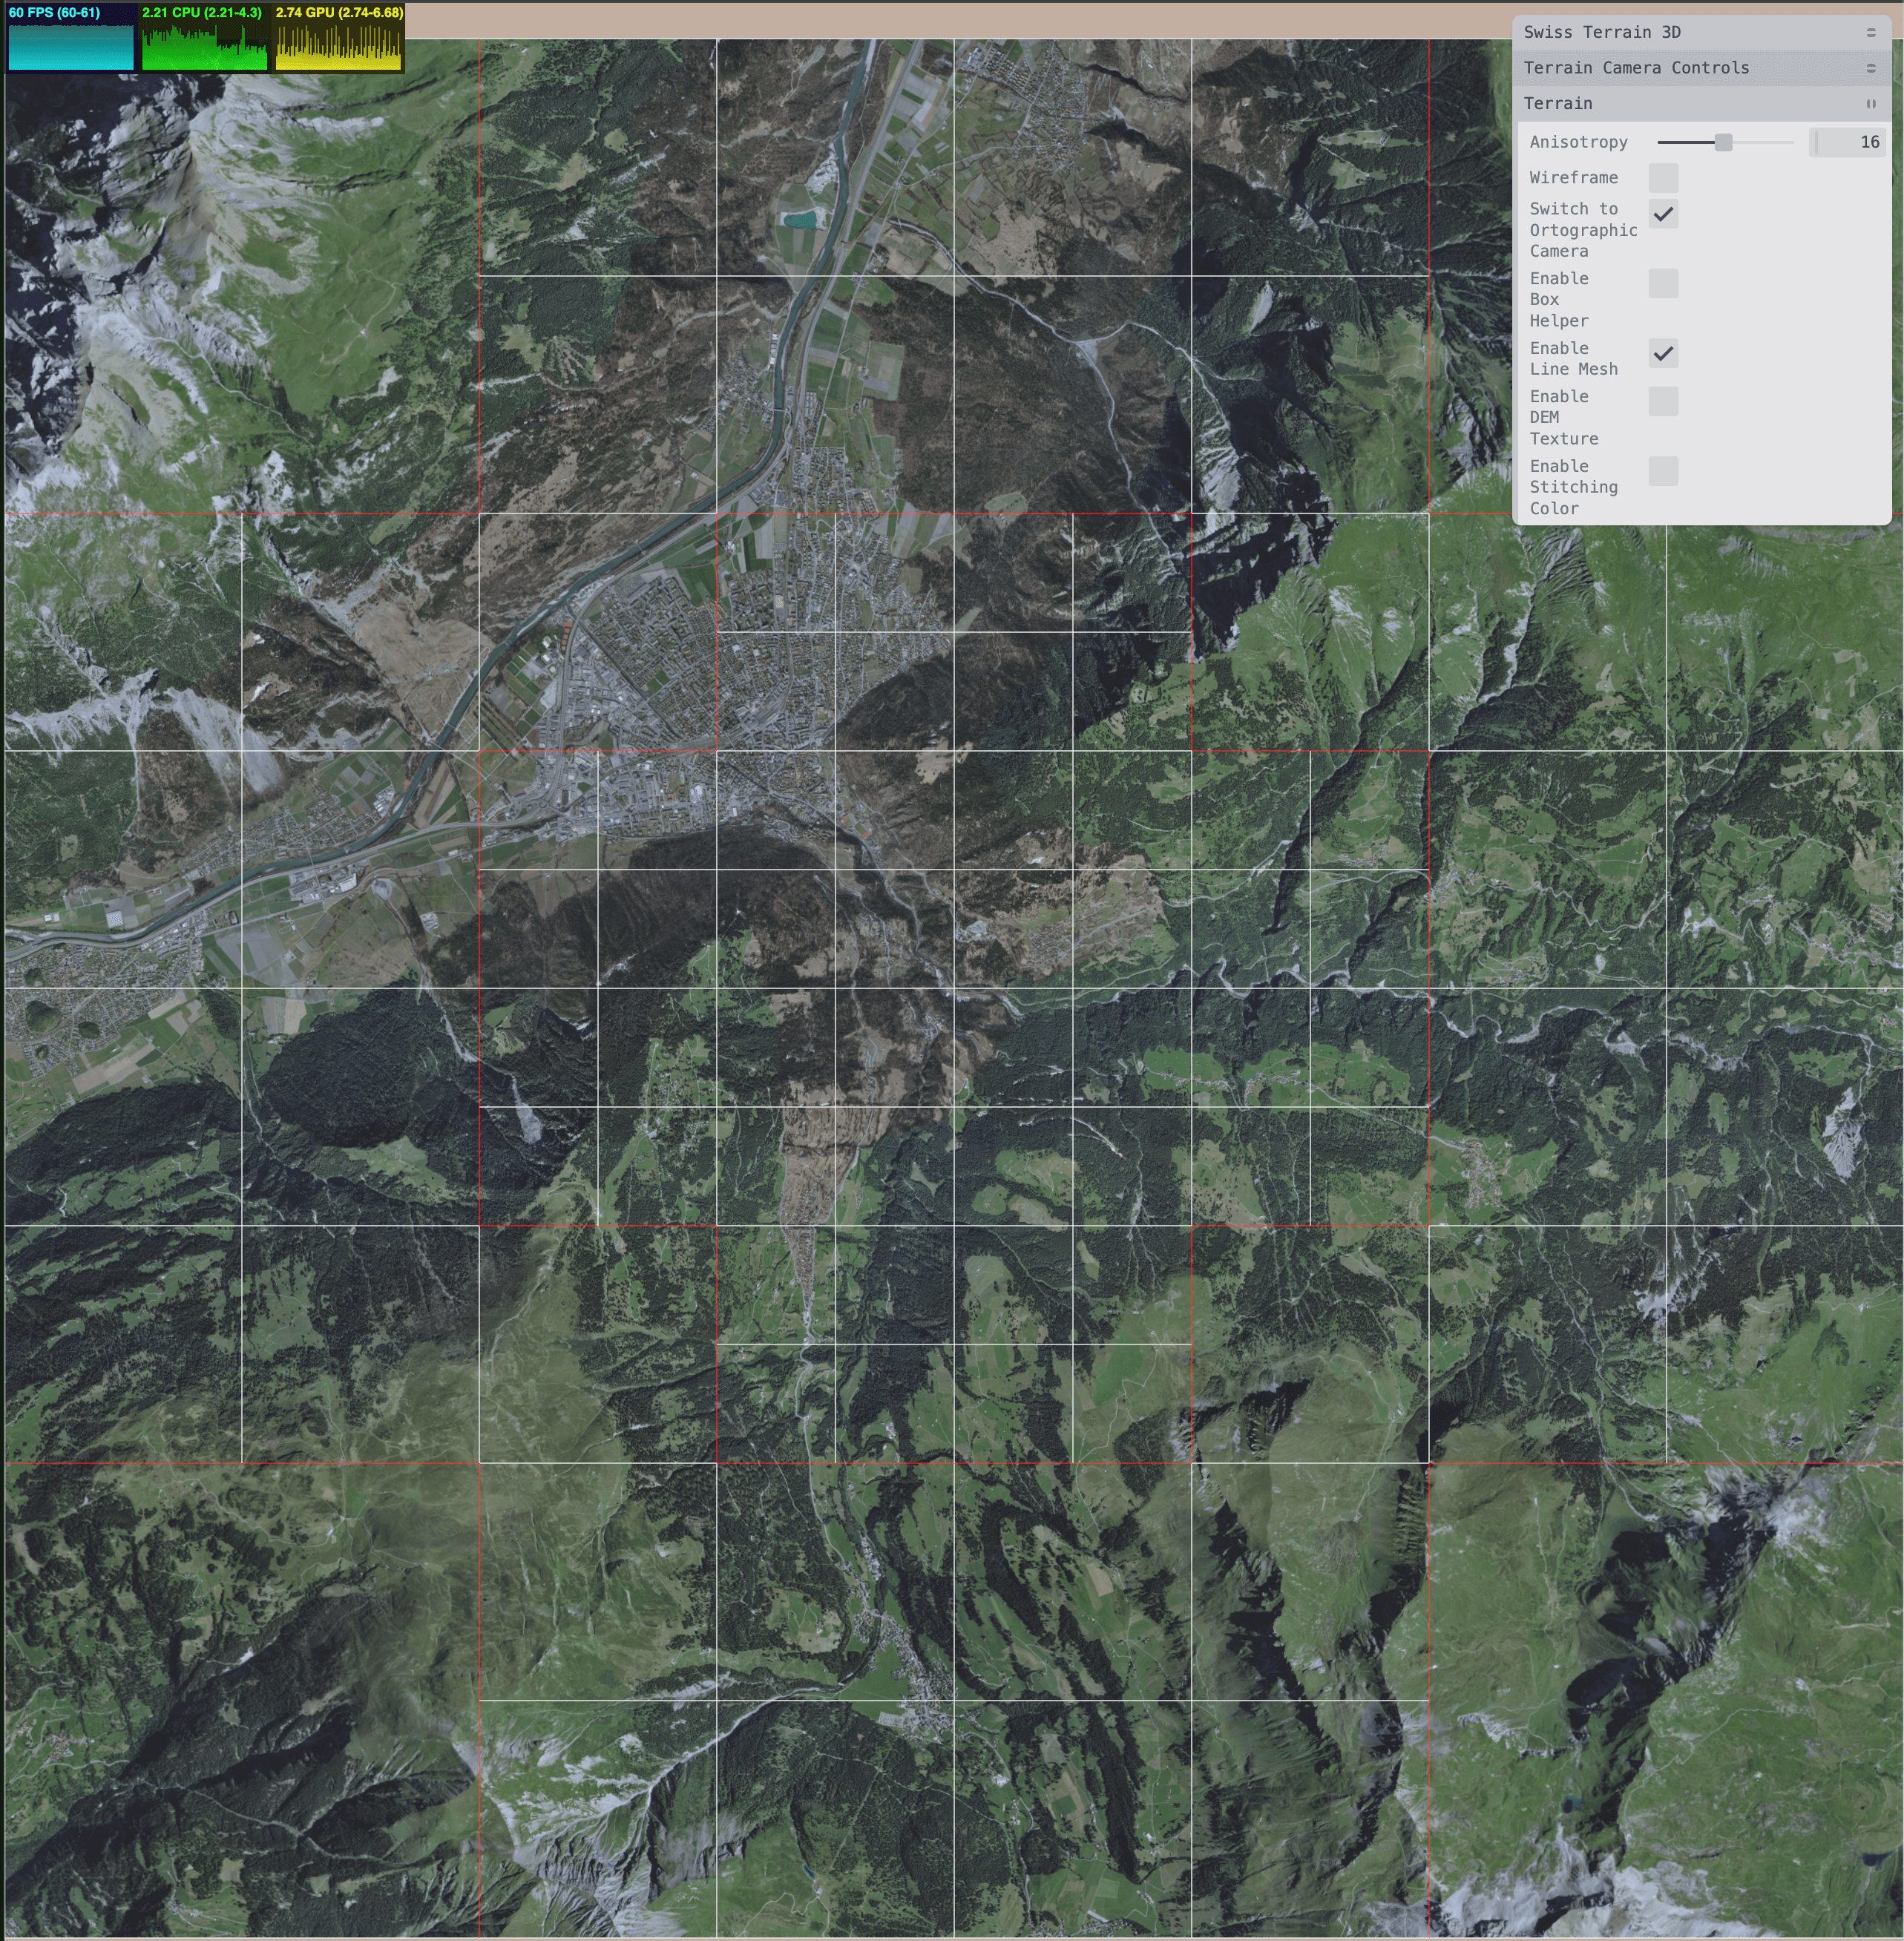
\includegraphics[width=.4\linewidth]{content/00_assets/hilfsvisualisierung_quadtree.png}
    \label{fig_hilfsvisualisierung_quadtree_index_stitching}
\end{figure}

\subsection{Steuerungselemente}
\label{chap_steuerungselemente}
Damit eine freie Bewegung durch das Gebirge möglich ist, müssen entsprechende Steuerungselemente implementiert werden. Der Betrachtungsausschnitt der Visualisierung wird durch eine Kamera definiert. In Three.js stehen verschiedene Arten von Kameras zur Verfügung. Eine ``Perspective Camera'' wird beispielsweise eingesetzt, um Objekte im 3D-Raum darzustellen. Dabei erscheinen die entsprechenden Objekte, abhängig von der Distanz zur Kamera, entsprechend grösser oder kleiner. Die ``Ortographic Camera'' stellt alle Objekte unabhängig von der Distanz gleich gross dar (siehe Abbildung \ref{fig_threejs_cameras}). Aus diesen Gründen wird für die Terrainvisualisierung eine Perspective Camera und für Hilfsvisualisierung eine Ortographic Camera verwendet. 
\begin{figure}[H]
    \caption{Verschiedene Arten von Kameras in Three.js \parencite{threejs_exploring_cameras_2023}}
    \includegraphics[width=.5\linewidth]{content/00_assets/threejs_cameras.png}
    \label{fig_threejs_cameras}
\end{figure}

Mittels Maus und Tastatur können sowohl die Position als auch der Betrachtungswinkel der Kameras verändert werden und erlauben somit eine freie Bewegung durch die Terrainvisualisierung. Tabelle \ref{table_steuerungselemente} zeigt eine Übersicht der Steuerungselemente und deren Auswirkung.
\begin{table}[H]
    \caption{Übersicht über Steuerungselemente und deren Auswirkung (Eigene Darstellung)}
    \begin{tabularx}{\textwidth} {
        >{\raggedright\arraybackslash}X 
        >{\raggedright\arraybackslash}X}
            \hline
            \textbf{Steuerungselement} & {Auswirkung}  \\
            \hline
            W-Taste oder Pfeiltaste nach oben & Bewegung nach vorne \\
            A-Taste oder Pfeiltaste nach link & Bewegung nach links \\
            S-Taste oder Pfeiltaste nach unten & Bewegung nach hinten \\
            D-Taste oder Pfeiltaste nach rechts & Bewegung nach rechts \\
            E-Taste & Bewegung nach oben \\
            R-Taste & Bewegung nach unten \\
            Mausbewegung & Veränderung des Betrachtungswinkels \\
            \hline
    \end{tabularx}
    \bigbreak
    \label{table_steuerungselemente}
\end{table}

\section{Ästhetik}
Three.js bietet diverse Möglichkeiten, um die Ästhetik einer 3D-Visualisierung zu beeinflussen. Ziel dieses Kapitels ist es, einen Überblick über die verwendeten ästhetischen Anpassungen sowie deren Einfluss zu erhalten.

\subsection{\acrfull{HDR} und Tone Mapping}
\acrfull{HDR} ermöglicht im Kontext digitaler Bilder eine feinere Darstellung des Helligkeitsspektrums. In herkömmlichen Bildformaten sind Farben nur innerhalb eines begrenzten Intensitätsbereichs unterscheidbar. Helle Bildbereiche werden weiss dargestellt, während dunkle Bereiche schwarz erscheinen. Dieser darstellbare Intensitätsbereich wird als Dynamic Range bezeichnet. Da HDR diesen Bereich deutlich erweitert und in feineren Abstufungen abbildet, können Helligkeitsunterschiede präziser dargestellt werden \parencite{hdr_2022}. Abbildung \ref{fig_terrain_hdr_no_hdr} veranschaulicht die resultierenden Kontrastunterschiede.

\begin{figure}[H]
    \caption{Kontrastunterschied der Gebirge mit HDR (links) und ohne (rechts) (Eigene Darstellung)}
    \includegraphics[width=1.0\linewidth]{content/00_assets/terrain_hdr_no_hdr.png}
    \label{fig_terrain_hdr_no_hdr}
\end{figure}

Um \acrshort{HDR} Bilder zu erstellen, gibt es mehrere Möglichkeiten. Einerseits können die Bilder mittels des Computers erstellt werden, andererseits ist es auch möglich ein \acrshort{HDR} Bild auf Basis von mehreren Einzelbildern mittels speziellen Kamerasensoren zu erstellen \parencite{hdr_2022}. Darüber hinaus gibt es spezialisierte Webseiten wie Poly Haven\footnote{\url{https://polyhaven.com/hdris}} womit HDR Bilder direkt heruntergeladen werden können.

Damit die Farbwerte von HDR Bildern auf dem Bildschirm dargestellt werden können, müssen sie in ein darstellbares Spektrum überführt werden. Um dies zu ermöglichen, wird das sogenannte ``Tone Mapping'' verwendet. Three.js unterstützt hierbei Tone Mapping-Verfahren. Abbildung \ref{fig_tone_mapping_threejs} zeigt die Auswirkungen von verschiedenen Tone Mapping-Verfahren auf die finale Darstellung.

\begin{figure}[H]
    \caption{Verschiedene Tone Mapping-Verfahren in Three.js von links nach rechts (kein Tone Mapping, Agx, Filmic, Reinhard) (Eigene Darstellung)}
    \includegraphics[width=.8\linewidth]{content/00_assets/tone_mapping_threejs.png}
    \label{fig_tone_mapping_threejs}
\end{figure}

\subsection{Anisotropy}
Um die Performance zu erhöhen, können für Texturen sogenannte ``Mipmaps'' erstellt werden. Mipmaps sind herunterskalierte Versionen der Originaltextur (siehe Abbildung \ref{fig_mipmaps}). Die Grafikkarte selektiert je nach Blickwinkel und Abstand die passende Mipmap Textur. Mit dieser Methode werden automatisch kleinere (herunterskalierte) Versionen für Dinge genutzt, welche sich in der Ferne befinden \parencite{mipmaps_2023}.
\begin{figure}[H]
    \caption{Mipmaps \parencite{mipmaps_2023}}
    \includegraphics[width=.3\linewidth]{content/00_assets/mipmaps.jpg}
    \label{fig_mipmaps}
\end{figure}

Es kann es bei der Verwendung von Mipmaps dazu führen, dass Texturen, welche sich in der Ferne befinden, kaum mehr erkennbar sind oder unscharf erscheinen. Um dieses Problem zu lösen, gibt es die Möglichkeit, über die sogenannten ``Anisotropy'' zu definieren, wie oft die einzelnen Bildpunkte einer Mipmap gefiltert werden sollen \parencite{threejs_anisotropy_2025}. Somit können verwaschene und unscharfe Texturen vermieden werden (siehe rote Bereiche A und B in Abbildung \ref{fig_anisotropy}).
\begin{figure}[H]
    \caption{Texturen mit Anisotropy (links) und ohne (rechts) (Eigene Darstellung)}
    \includegraphics[width=1.0\linewidth]{content/00_assets/textur_mit_anisotropy_ohne.png}
    \label{fig_anisotropy}
\end{figure}

\subsection{Procedural Sky}
Das Three.js-Ökosystem stellt zahlreiche Module zur Verfügung, um realitätsnahe Visualisierungen zu erzeugen. Ein Beispiel hierfür ist das \textit{Procedural Sky Plugin}\footnote{\url{https://threejs.org/examples/?q=sky#webgpu_sky}}, mit dem sich ein Tag-Nacht-Zyklus simulieren lässt. Das Plugin bietet verschiedene Einstellungsmöglichkeiten, etwa zur Definition der Sonnenposition, wodurch das dargestellte Gebirge in eine realitätsnahe Lichtumgebung eingebettet werden kann. Abbildung \ref{fig_procedural_sky} veranschaulicht den Einfluss auf die Darstellung des Gebirges anhand unterschiedlicher Sonnenpositionen. 
\begin{figure}[H]
    \caption{Gebirge mit Procedural Sky Plugin (Eigene Darstellung)}
    \includegraphics[width=1.0\linewidth]{content/00_assets/threejs_procedural_sky.png}
    \label{fig_procedural_sky}
\end{figure}

\subsection{Einstellungsmöglichkeiten}
Die bislang behandelten ästhetischen Elemente verfügen über eine Vielzahl einstellbarer Parameter. Um deren Auswirkungen auf die visuelle Gestaltung nachvollziehen zu können, ist es wichtig, dass diese Parameter während der Laufzeit über geeignete GUI-Elemente angepasst werden können. Um Einstellungsparameter mit entsprechenden GUI-Elementen zu verknüpfen, stehen diverse Bibliotheken zur Verfügung. Eine populäre Bibliothek in der Three.js-Community ist Tweakpane\footnote{\url{https://tweakpane.github.io/docs/}}. Tweakpane bietet eine Vielzahl von unterschiedlichen GUI-Elementen wie Range-Slider, Color-Picker oder Accordions an. Tweakpane stellt zudem eine einheitliche Darstellung dieser Elemente zwischen den einzelnen Browsern sicher und ermöglicht es ebenfalls, die Elemente mithilfe von Themes\footnote{\url{https://tweakpane.github.io/docs/theming/}} entsprechend anzupassen. Der zentrale Vorteil von Tweakpane gegenüber standardmässigen HTML5-GUI-Elementen liegt in der unkomplizierten Verknüpfung von Einstellungsparametern mit den entsprechenden Bedienelementen. Zur Erstellung eines Dropdown-Menüs für die Auswahl des Tone-Mappings müssen lediglich die verfügbaren Optionen sowie die auszuführende Aktion beim Selektieren eines Eintrags definiert werden (siehe Abbildung \ref{fig_tweaks_code}).
\begin{figure}[H]
    \caption{Definitionsstruktur für ein Dropdown in Tweakpane (Eigene Darstellung)}
    \includegraphics[width=.6\linewidth]{content/00_assets/tweaks_beispiel_code.png}
    \label{fig_tweaks_code}
\end{figure}

Dies ermöglicht es, schnell neue Bedienelemente für zentrale Parameter zu konfigurieren. Abbildung \ref{fig_tweaks} zeigt eine Auswahl von GUI-Elementen (Tweaks), mit denen verschiedene Aspekte der Terrain-Visualisierung in Echtzeit angepasst werden können.
\begin{figure}[H]
    \caption{Tweaks der Terrain-Visualisierung (Eigene Darstellung)}
    \includegraphics[width=.3\linewidth]{content/00_assets/tweaks.png}
    \label{fig_tweaks}
\end{figure}

\section{Performanz}
Im Rahmen dieses Kapitels wird die Leistungsfähigkeit der Visualisierung evaluiert. Davon ausgehend werden entsprechende Engpässe aufgedeckt und durchgeführte Optimierungen besprochen. Die Messung erfolgte auf einem Macbook Pro M3 Max mit 64GB Arbeitsspeicher. Als Gebirge wurde der Raum Chur über ein Gebiet von 16 km$^2$ verwendet. 

\subsection{Im Vorfeld vorgenommene Optimierungen}
Vor der eigentlichen Messung wurden bereits einige Optimierungen im Vorfeld vorgenommen. Nachfolgend wird kurz auf die wichtigsten Optimierungen eingegangen.

\subsubsection{Webworker für Quadtree-Algorithmus}
Webbrowser führen JavaScript-Code standardmässig in einem einzelnen Thread aus. Dadurch können rechenintensive Operationen die Visualisierung blockieren und zu wahrnehmbaren Verzögerungen führen. Durch den Einsatz von sogenannten ``Webworkern'' lassen sich solche Berechnungen in separate Threads auslagern und im Hintergrund ausführen. Web Worker besitzen keinen Zugriff auf das \acrfull{DOM} des Browsers, wodurch unter anderem das direkte Laden von Texturen nicht möglich ist. Dennoch eignen sie sich für die Auslagerung rechenintensiver Algorithmen wie des Quadtrees. Auf diese Weise können sowohl die Berechnung als auch das Ausbalancieren des Quadtrees im Hintergrund erfolgen, während sich der Main-Thread auf die Aktualisierung und Darstellung der daraus abgeleiteten 3D-Modelle konzentriert.

\subsubsection{Vorladen der Texturen}
Um ein dynamisches Nachladen der Texturen einzelner Quadtree-Nodes zu vermeiden, werden diese bereits beim Start der Applikation vorgeladen. Zwar führt dies initial zu einer längeren Ladezeit, während der Laufzeit stehen die Texturen jedoch unmittelbar zur Verfügung, sodass Ladeverzögerungen vermieden werden.

\subsubsection{Frustum Culling}
Wie in Kapitel \ref{chap_steuerungselemente} beschrieben, unterstützt Three.js verschiedene Kameratypen, die jeweils ein definiertes Sichtfeld (Frustum) besitzen. Um Rechenleistung zu sparen, werden Objekte ausserhalb dieses Sichtfeldes nicht gezeichnet. Dieses Verfahren wird als ``Frustum Culling'' bezeichnet. Zur Bestimmung, ob sich ein Objekt innerhalb oder ausserhalb des Sichtfeldes befindet, verwendet Three.js sogenannte ``Bounding Spheres''. Diese werden zur Laufzeit für jede Geometrie berechnet. Grundlage hierfür ist eine ``Bounding Box'', also ein dreidimensionaler Bereich, der die jeweilige Geometrie vollständig umschliesst (siehe rote markierte Bereiche in Abbildung \ref{fig_bounding_boxes}).
\begin{figure}[H]
    \caption{Visualisierung der Bounding Box (Eigene Darstellung)}
    \includegraphics[width=.4\linewidth]{content/00_assets/terrain_bounding_boxes.png}
    \label{fig_bounding_boxes}
\end{figure}
Die Bounding Box wird aufgrund der globalen Höhenwerte des Gebirges sowie der räumlichen Abdeckung der Quadtree Nodes berechnet. Auf Basis dieses Bereiches kann anschliessend die für das Frustum Culling notwendige Bounding Sphere berechnet werden (siehe Abbildung \ref{fig_berechnung_bounding_box}).

\begin{figure}[H]
    \caption{Berechnung der Bounding Box (Eigene Darstellung)}
    \includegraphics[width=.5\linewidth]{content/00_assets/berechnung_bbox.png}
    \label{fig_berechnung_bounding_box}
\end{figure}

\subsubsection{Vorberechnung der Geometrie}
Die grundlegende Geometrie aller Quadtree-Nodes ist identisch und unterscheidet sich lediglich in ihrer Grösse sowie in der jeweils verwendeten Index-Stitching-Variante (siehe Kapitel \ref{chap_visuelle_diskrepanz_zwischen_nodes}). Dadurch genügen neun vordefinierte Grundgeometrien, jeweils eine pro Index-Stitching-Variante, um das gesamte Gebirge darzustellen. Um aufwendige Berechnungen während der Laufzeit zu vermeiden, werden diese Geometrien bereits beim Start der Applikation vorberechnet. Während der Laufzeit müssen sie anschliessend lediglich den entsprechenden Quadtree-Nodes zugewiesen sowie passend positioniert und skaliert werden.

\subsection{Messung}
Die Messung orientiert sich an den in Kapitel \ref{technologie_anforderungen} erwähnten Anforderungen. Um die Bildwiederholrate als auch diverse andere wichtige Faktoren wie CPU- und GPU-Auslastung zu überwachen, wird die Bibliothek stats-gl\footnote{\url{https://github.com/RenaudRohlinger/stats-gl}} verwendet. Ein Vorteil von stats-gl ist die einfache Integration in das Three.js Framework. In einem ersten Schritt werden die Metriken definiert, welche gemessen werden sollen (siehe \textit{trackFPS} und \textit{trackGPU} in Abbildung \ref{fig_statsgl}). Anschliessend wird stats-gl initialisiert und periodisch aktualisiert.

\begin{figure}[H]
    \caption{Integration von stats-gl in Three.js (Eigene Darstellung)}
    \includegraphics[width=.4\linewidth]{content/00_assets/statsgl.png}
    \label{fig_statsgl}
\end{figure}

Richtig konfiguriert erlaubt stats-gl die Überwachung der vordefinierten Metriken in Echtzeit. Die Metriken werden in Form von verschiedenen Grafen dargestellt (siehe Abbildung \ref{fig_threejs_statsgl}). Beim Ablesen der Grafen hat sich gezeigt, dass die definierten Zielmetriken in Bezug auf Auflösung und Bildwiederholrate prinzipiell erreicht werden konnten. 
\begin{figure}[H]
    \caption{Grafwidgets von stats-gl (Eigene Darstellung)}
    \includegraphics[width=.4\linewidth]{content/00_assets/threejs_statsgl.png}
    \label{fig_threejs_statsgl}
\end{figure}

\subsection{Identifikation von Engpässen}
Während der Navigation durch ein grösseres Gebirge, konkret die Region Chur, konnten insbesondere beim Einsatz des neuen WebGPU-Backends von Three.js kurze Unterbrechungen beobachtet werden. Diese treten jeweils dann auf, wenn neue Geometrien erzeugt werden. Mithilfe der integrierten Browser-Entwicklungswerkzeuge zeigte sich, dass rund 60\% der Laufzeit auf die Methode\textit{build} entfallen (siehe Abbildung \ref{fig_webgpu_build_issue}). 
\begin{figure}[H]
    \caption{WebGPU Engpass in \textit{build} Methode (Eigene Darstellung)}
    \includegraphics[width=.5\linewidth]{content/00_assets/performance_issue_build_method.png}
    \label{fig_webgpu_build_issue}
\end{figure}

Diese Methode übersetzt den \acrshort{TSL} spezifischen Code (siehe Kapitel \ref{chap_erstellung_geometrie}) in die jeweilige Shadersprache (GLSL bzw. WGSL). Die Übersetzung erfolgt auf der CPU und kann bei längeren Ausführungszeiten zu Leistungsengpässen führen. Beim WebGL-Backend entfällt dieser Schritt, da der Shader-Code direkt in GLSL verfasst wird. Ein weiterer Engpass, der sowohl im WebGPU- als auch im WebGL-Backend beobachtet wurde, ist das Dekodieren von Bilddateien. Abbildung \ref{fig_performance_issue_image_decode} zeigt, dass im WebGL-Backend hierfür rund 40\% der gesamten Ausführungszeit aufgewendet werden. 
\begin{figure}[H]
    \caption{Dekodieren der Bilddateien (Eigene Darstellung)}
    \includegraphics[width=.8\linewidth]{content/00_assets/performance_issue_image_decode.png}
    \label{fig_performance_issue_image_decode}
\end{figure}

\subsection{Optimierungen}
Zur Behebung der Übersetzungsproblematik wurde entschieden, das WebGL-Backend anstelle des WebGPU-Backends einzusetzen. Three.js unterstützt den Wechsel des Backends, sodass grosse Teile des bestehenden Codes weiterverwendet werden konnten. Lediglich der Shader-Code musste im Zuge der Umstellung von TSL auf GLSL angepasst werden (siehe Abbildung \ref{fig_vertex_shader_glsl_tsl}).
\begin{figure}[H]
    \caption{Unterschiede zwischen GLSL und TSL Code (Eigene Darstellung)}
    \includegraphics[width=.6\linewidth]{content/00_assets/terrain_vertex_shader_glsl_tsl.png}
    \label{fig_vertex_shader_glsl_tsl}
\end{figure}

Um Bilddaten direkt auf der Grafikkarte nutzen zu können, stehen spezielle, GPU-optimierte Bildformate zur Verfügung. Eines dieser Formate ist \acrfull{KTX}\footnote{\url{https://github.khronos.org/KTX-Specification/ktxspec.v2.html}}. KTX-Bilder liegen bereits in einem für die Grafikhardware geeigneten Format vor und müssen daher nicht mehr dekodiert werden. Hierfür wurde die Datenvorverarbeitung angepasst, sodass die Texturen zusätzlich im optimierten KTX-Format erzeugt werden.

\subsubsection{Zukünftige Optimierungsmöglichkeiten}
\label{chap_future_optimizations}
Mit Analysewerkzeugen wie SpectorJS\footnote{\url{https://spector.babylonjs.com}} lässt sich jedes einzelne Bild detailliert auf der Grafikkarte untersuchen. Dabei zeigt sich, dass für jede Geometrie ein eigener Draw Call an die Grafikkarte gesendet wird. Für die Region Chur sind entsprechend rund 89 Draw Calls erforderlich (siehe Abbildung \ref{fig_spectorjs_draw_calls}). Diese Anzahl steigt mit der Zahl der Quadtree-Nodes und damit mit der Grösse des dargestellten Gebirges. Insbesondere auf leistungsschwächeren Endgeräten, etwa Smartphones, kann dies zu Leistungsengpässen führen. 
\begin{figure}[H]
    \caption{SpectorJS Anzahl Draw Calls für Raum Chur (Eigene Darstellung)}
    \includegraphics[width=.3\linewidth]{content/00_assets/spectorjs_draw_calls.png}
    \label{fig_spectorjs_draw_calls}
\end{figure}
Three.js bietet mit dem sogenannten ``Instance Rendering'' eine Lösung für dieses Problem. Dieses Verfahren ermöglicht es, eine grosse Anzahl identischer Geometrien innerhalb eines einzelnen Draw Calls zu zeichnen. Voraussetzung ist, dass alle Instanzen dieselbe Geometrie verwenden (siehe Abbildung \ref{fig_threejs_instance_rendering}). Da für die Terrain-Visualisierung lediglich neun unterschiedliche Geometrievarianten existieren, lässt sich hiermit die Anzahl der benötigten Draw Calls erheblich reduzieren.
\begin{figure}[H]
    \caption{Three.js Instance Rendering \parencite{threejs_instance_rendering_2025}}
    \includegraphics[width=.4\linewidth]{content/00_assets/threejs_instance_rendering.png}
    \label{fig_threejs_instance_rendering}
\end{figure}
